\documentclass[12pt,a4paper]{report}
\setcounter{secnumdepth}{5} % setting level of numbering (default for "report" is 3).
\usepackage{natbib}
\usepackage[utf8]{inputenc}
\usepackage[french]{babel}
\usepackage[T1]{fontenc}
\usepackage{amsmath}
\usepackage{amsfonts}
\usepackage{amssymb}
\usepackage{graphicx}
\usepackage{appendix}
\usepackage{enumitem}
\usepackage{float} 
\usepackage[nottoc, notlof, notlot]{tocbibind}
\usepackage{pdfpages}
\usepackage{gensymb}
\usepackage{lipsum}
\usepackage[colorinlistoftodos,textwidth=3.7cm]{todonotes}
\usepackage[top=1in, bottom=1in, left=1in, right=1in]{geometry}
\usepackage{tocbibind}
\usepackage[hidelinks]{hyperref}
\usepackage[justification=centering]{caption}
\usepackage[acronym]{glossaries}
\usepackage{listings}
\author{Sébastien Hervieu}

\setcounter{MaxMatrixCols}{20}
\newcounter{mypagecount}% create a new counter
\setcounter{mypagecount}{0}% set it to something just in case
\newenvironment{interlude}{% create a new environment for the unnumbered section(s)
	\clearpage
	\setcounter{mypagecount}{\value{page}}% use the new counter we created to hold the page count at the start of the unnumbered section
	\thispagestyle{empty}% we want this page to be empty (adjust to use a modified page style)
	\pagestyle{empty}% use the same style for subsequent pages in the unnumbered section
}{%
	\clearpage
	\setcounter{page}{\value{mypagecount}}% restore the incremented value to the official tally of pages so the page numbering continues correctly
}

\newglossaryentry{utc}{name=utc,description={Coordinated Universal Time}}
\newglossaryentry{adt}{name=adt,description={Atlantic Daylight Time}}
\newglossaryentry{est}{name=est,description={Eastern Standard Time}}
\newacronym{cd}{CD}{compact disk}

\makeglossaries

\lstset{
	numbers=left, 
	numberstyle=\small, 
	numbersep=8pt, 
	frame = single,  
	framexleftmargin=15pt}

%from documentation
%\newacronym[⟨key-val list⟩]{⟨label ⟩}{⟨abbrv ⟩}{⟨long⟩}
%above is short version of this
% \newglossaryentry{⟨label ⟩}{type=\acronymtype,
% name={⟨abbrv ⟩},
% description={⟨long⟩},
% text={⟨abbrv ⟩},
% first={⟨long⟩ (⟨abbrv ⟩)},
% plural={⟨abbrv ⟩\glspluralsuffix},
% firstplural={⟨long⟩\glspluralsuffix\space (⟨abbrv ⟩\glspluralsuffix)},
% ⟨key-val list⟩}



%\newglossaryentry{tree}{name={tree},description={trees are the better humans}}


\begin{document}
	
\newcommand{\para}{\paragraph*{}}

\newcommand{\bs}[1]{\boldsymbol{#1}}
	
\newcommand{\todoRediger}[1]{\todo[color=red,inline]{REDIGER #1}}
\newcommand{\todoARevoir}[1]{\todo[color=red,inline]{A REVOIR #1}}
\newcommand{\todoCompleter}[1]{\todo[inline]{COMPLETER #1}}
\newcommand{\todoAmeliorer}[1]{\todo{AMELIORER: #1}}
\newcommand{\todoMiseEnForme}[1]{\todo[color=green,inline]{MISE EN FORME: #1}}
\newcommand{\todoCheck}[1]{\todo[color=cyan,fancyline]{VERIFIER #1}}
\newcommand{\todoAjouterRef}[1]{\todo[color=pink]{AJOUTER REF #1}}
\newcommand{\todoTrouverRefExt}[1]{\todo[color=red,inline]{TROUVER REF EXTERNE: #1}}
\newcommand{\todoObjectif}[1]{\todo[color=yellow,inline,size=\Large]{OBJECTIF: #1}}
\newcommand{\todoPeutEtre}[1]{\todo[color=teal,inline]{PEUT ETRE #1 ?}}

\begin{titlepage}

\newcommand{\HRule}{\rule{\linewidth}{0.5mm}} % Defines a new command for the horizontal lines, change thickness here

\center % Center everything on the page
 
%----------------------------------------------------------------------------------------
%	HEADING SECTIONS
%----------------------------------------------------------------------------------------

\textsc{\LARGE Université de Rennes 1}\\[1cm] 
\textsc{\Large }\\[0.5cm] % Major heading such as course name
\textsc{\large Master 2 Calcul scientifique et modélisation}\\
\textsc{Rapport de Stage}\\
%----------------------------------------------------------------------------------------
%	TITLE SECTION
%----------------------------------------------------------------------------------------

\HRule \\[0.4cm]
{ \huge \bfseries Etude et développement d’outils mathématiques pour estimer, en temps réel, le tassage et le volume d’un silo de maïs à partir de capteurs embarqués}\\[0.4cm] 
\HRule \\[1.5cm]
 
%----------------------------------------------------------------------------------------
%	AUTHOR SECTION
%----------------------------------------------------------------------------------------

\begin{minipage}{0.4\textwidth}
\begin{flushleft} \large
\emph{Auteur:}\\
Sébastien \textsc{Hervieu}
\end{flushleft}
\end{minipage}
~
\begin{minipage}{0.4\textwidth}

\begin{flushright}
	\emph{Tuteur de Stage:} \\
	Geoffroy \textsc{Etaix}
\end{flushright}

\begin{flushright} \large
	\emph{Tuteur Universitaire:} \\
	Fabrice \textsc{Mahé} 
\end{flushright}

\end{minipage}\\[1cm]

% If you don't want a supervisor, uncomment the two lines below and remove the section above
%\Large \emph{Author:}\\
%John \textsc{Smith}\\[3cm] % Your name

%----------------------------------------------------------------------------------------
%	DATE SECTION
%----------------------------------------------------------------------------------------

{\large \today}\\[1cm] % Date, change the \today to a set date if you want to be precise

%----------------------------------------------------------------------------------------
%	LOGO SECTION
%----------------------------------------------------------------------------------------
\includegraphics[height=3cm]{img/logo-tellusenv.png} \\
\includegraphics[height=3cm]{img/univ.jpeg}\\[1cm] % Include a department/university logo - this will require the graphicx package
 
%----------------------------------------------------------------------------------------

\vfill % Fill the rest of the page with whitespace

\end{titlepage}


%\begin{interlude}
%\listoftodos
%\end{interlude}

\cleardoublepage% especially in a document where chapters start at right-hand pages
%\phantomsection% for an anchor if you use hyperref

\chapter*{Remerciements}% for the actuall unnumbered heading
\addcontentsline{toc}{chapter}{\numberline{}Remerciements}% if you wish to have a TOC entry
\thispagestyle{empty}% or plain etc.
\markboth{Remerciements}{Remerciements}% relevant depending on page style
% or if it's more than one page

\para Je tiens tout d'abord à remercier très sincèrement monsieur Geoffroy ETAIX, qui m'a accordé sa confiance pour mener ce stage, ainsi que toute l'équipe de Tellus Environment dont l'accueil et la gentillesse a été au dela de toutes mes espérances.

\para J'adresse mes remerciements respectueux à messieurs Fabrice Mahé et Eric Darrigrand, professeurs de l'Université de Rennes 1, qui m'ont permis de rejoindre cette formation et qui m'ont accompagné lors de la recherche de stage et de son  déroulement.

\para Je remercie le Fongecif Bretagne, dont le soutient m'a permis de réaliser ce congé de formation, ainsi que toute l'équipe d'IDAPPS qui m'a aidé dans le montage du dossier de financement: Stéphane RENGER, Yann GIRARDEAU et surtout Laila BENLARIBI, que je salue très chaleureusement. Qu'elle soit ici félicitée de sa redoutable efficacité! 

\para Je remercie l'équipe du service Formation Continue de l'Université Rennes I, mesdames Lisa GENDREAU et Marie-Gisèle DARAS

\para Je remercie enfin ma petite famille, mon épouse Céline et mes deux filles Clémentine et Angèle, pour leurs encouragements, leur soutien et leur patience tout au long de ces deux dernières années. Nous sommes sur un beau chemin.


\setcounter{tocdepth}{5}
\tableofcontents

\printglossaries

\chapter{Introduction}

J'effectue depuis le 3 avril 2018 mon stage de fin d'étude de Master 2 CSM au sein de Tellus Environnement, afin de mener à bien la partie étude et développement du projet appelé en interne "Symeter V2". Le but de ce projet est de permettre le monitoring du tassage d'un silo de maïs en temps réel en utilisant un LIDAR embarqué sur un tracteur.

\para Cette introduction présente les activités de Tellus Environment et introduit le contexte du projet Symeter V2. 

	\section{Tellus Environment - Missions Principales}

	\subsection{Géophysique et cartographie haute-définition}
	Tellus Environment a été créée en 2012 et s'est initialement spécialisée dans le traitement de données géophysiques, la cartographie haute définition des sous-sols et des fond-marins. Elle propose à ses clients une offre bout en bout d'acquisition et de traitement des données pour permettre à ses clients d'agir en fonction de ces conclusions.
	
	\subsection{Traitement des données}
	Tellus Environment dispose d'une expertise particulière du traitement des données géophysiques et optiques en mettant en oeuvre le procédé MagSalia, procédé dont le brevet est exploité exclusivement par l'entreprise.
	
	\para Initialement développé par le laboratoire de Mathématiques de L'Université de Bretagne Occidentale, ce procédé peut exploiter des mesures magnétiques, sonar multibeam ou LIDAR. Lorsqu'il est appliqué à des acquisitions magnétiques, il produit une tomographie en 3 dimensions de masses magnétiques ponctuelles et étendues jusqu'à 30 mètres de profondeur.
	
	\para Dans sa version sonar multifaisceaux ou LIDAR, il permet d'accentuer le relief du modèle numérique en mettant en évidence les anomalies du fond marin ou les perturbations de la sous-couche terrestre. Ceci est particulièrement adapté aux problématiques agricoles, archéologiques et aux divers aménagements qui nécessitent des zones vierges (non exploitées) ou blanches (exploitées mais cartographie imprécise ou absente).
	
	\subsection{Collecte des données géophysiques}
	
	\para Tellus Environment met en oeuvre également ses propres équipements géoradar et magnétomètre pour l'acquisition de données sur le sous-sol, sur des surfaces de quelques mètres-carrés à quelque hectares. Elle est aussi en mesure de planifier et coordonner la mise en oeuvre d'équipements plus lourds - LIDAR, géoradar (fig. \ref{fig:georadar} et \ref{fig:radargram}), magnétomètres aéroportés - pour obtenir des données sur des surfaces beaucoup plus importantes, de l'ordre du kilomètre carré.
	
	\begin{figure}
		\centering
		
		\begin{minipage}{.5\textwidth}
			\centering
			\includegraphics[width=0.7\linewidth]{img/IMG_0332}
			\caption[Géoradar]{Géoradar ZOND}
			\label{fig:georadar}
		\end{minipage}%
		\begin{minipage}{.5\textwidth}
				\centering
			\includegraphics[width=0.7\linewidth]{img/sonar}
			\caption[sonar]{Sonar (en cours d'utilisation)}
			\label{fig:sonar}
		\end{minipage}
	\end{figure}
	
	\begin{figure}
		\centering
		\includegraphics[width=0.7\linewidth]{img/radargram}
		\caption[radargramme]{Exemple d'un radargramme d'une détection \hspace{\textwidth} de réseaux enterrés. (Image Tellus Environment)}
		\label{fig:radargram}
	\end{figure}
	
	\para Tellus Environment peut aussi coordonner le déploiement d'équipements d'acquisition marins - sonar (fig. \ref{fig:sonar} et \ref{fig:e1790}), multibeam, etc - pour permettre la cartographie des fonds marins et des sous-sols aquatiques, que ce soit en environnement eau douce - rivières, lacs étangs - ou marins. 
	
	\begin{figure}
		\centering
		\includegraphics[width=0.7\linewidth]{img/E1790}
		\caption[sonargramme]{Exemple d'un sonargramme généré par un sonar sub-bottom (Image Tellus Envirinment)}
		\label{fig:e1790}
	\end{figure}

	
	\para Tellus Environment est spécialiste de la fusion de données (géophysiques et optiques), en ayant accès à de nombreuses bases cartographiques pour extraire l'information utile sur une zone d'intérêt.


	\section{Activité R\&D}
	
	Tellus Environment comprend une activité R\&D de cartographie qui met en oeuvre ses expertises en traitement de données, en capteurs liés à la géophysique pour participer au développement de produits innovants.
	
	\para Le sujet de ce stage se déroule au sein de l'activité R\&D de Tellus Environment pour participer au développement du projet Symeter V2.

	\section{Projet Symeter V2}
	Le projet Symeter V2 constiste en la mise en oeuvre de LIDARs montés sur un tracteur de tassage de silo maïs, en vue de mesurer en temps réel la qualité de tassage du maïs. Ce projet prend la suite du Symeter V1 qui est décrit dans la section suivante.
	
		\subsection{Symeter V1}
		\label{sec:symeterv1}
		Symeter V1 est un équipement qui permet de mesurer en temps réel l'état de tassage d'un silo de fourrage (maïs, herbe, ...) en vue d'augmenter la qualité des silos générés. Il est basé sur un équipement de mesure laser, le LIDAR, qui permet de collecter très rapidement de nombreux points de mesure. 
		
		\para Ce LIDAR est placé à l'aplomb du silo, au sommet d'une perche de 7m de hauteur, stabilisée par un trépied (voir fig. \ref{fig:symeterv1}). La visualisation des données est transmise au moyen d'une liaison WIFI à un écran embarqué dans le tracteur de tassage (fig. \ref{fig:archigenv1}).
		
		\begin{figure}[h!]
			\centering
			\includegraphics[width=0.6\linewidth]{img/ArchiGenV1}
			\caption[archisymv1]{Architecture de Symeter V1}
			\label{fig:archigenv1}
		\end{figure}
		
		
		\begin{figure}[h!]
			\centering
			\includegraphics[width=0.6\linewidth]{img/symeterv1}
			\caption[symeterv1]{Le système Symeter V1 en cours d'utilisation}
			\label{fig:symeterv1}
		\end{figure}
		
		
		\para Ce produit a été développé dans le courant de l'année 2017. Son utilisation sur des chantiers d'ensilage réel avait démontré que la mesure de tassage était possible et précise. Mais le retour d'expérience a mis en évidence des points d'amélioration.
		
		\para Tout d'abord, le déploiement et la configuration de l'installation est plutôt longue et complexe, ce qui n'est adapté pas à la contrainte de mise en oeuvre simple et rapide qui est généralement demandée pour les outils de chantiers d'ensilage.
		
		\para Ensuite des problèmes de connectivité dans la liaison sans fil entre le module d'acquisition et de traitement d'une part, et la tablette chargée de l'affichage des informations d'autre part, induisent une fiabilité aléatoire du système.
		
		\para Enfin le positionnement du trépied au plus près du silo en vue d'en obtenir un point de vue le plus à l'aplomb possible (voir fig. \ref{fig:symeterv1}) pose un risque non négligeable de collision entre le tracteur de tassage et le trépied. Cette collision forcerait le re-déploiement du trépied.
		

		\subsection{Symeter V2: Objectifs}
		Le projet Symeter V2 a donc été lancé pour améliorer Symeter V1 en prenant en compte des retours d'expérience exposés dans la section \ref{sec:symeterv1}. Un choix radical était nécessaire pour permettre à la fois la simplicité de mise en oeuvre, réduire le nombre de composants en interaction et limiter le besoin de liaisons sans fil. 
		
		\begin{figure}[h!]
			\centering
			\includegraphics[width=0.6\linewidth]{img/LidarMobile}
			\caption[archiv2]{Architecture de Symeter V2}
			\label{fig:lidarmobile}
		\end{figure}
		
		\para Il a donc été décidé de baser Symeter V2 sur le montage de l'équipement directement sur le tracteur de tassage, comme indiqué dans la figure \ref{fig:lidarmobile}. Cette configuration a pour avantage qu'elle supprime complètement le besoin d'une liaison sans fil. Tous les composants étant montés sur le tracteur, ils peuvent tous étre interconnectés au moyen de connections filaires.
		
		\para Le fait de monter une bonne fois pour toute l'équipement sur le tracteur permet d'avoir un déploiement sur chantier grandement simplifié, la calibration et la configuration étant effectuée en atelier lors du montage sur le tracteur. La mise en oeuvre de Symeter V2 par un simple appui sur un bouton au début du chantier d'ensilage est donc envisageable.
		
		\para Bien sûr le fait de monter un LIDAR sur une plateforme entraîne un besoin implicite fort: la \textit{pose} du tracteur doit être connue avec une assez grande précision à chaque instant pour permettre la construction du modèle numérique 3D du chantier d'ensilage. (la \textit{pose} d'un object dans un référentiel donnée est l'union de ses coordonnées Cartésiennes $x,y,z$ et des coordonnées angulaires de son attitude $\theta_x, \theta_y, \theta_z$ ).
		
		\para Ce nouveau besoin force la mise en oeuvre de capteurs et des méthodologies associées permettant de déterminer cette pose. Ces capteurs seront un IMU - une centrale intertielle miniaturisée - et un GPS exploité en mode RTK, appelé aussi "GPS centimétrique".
		
		\para La mise en oeuvre de ces capteurs pour déterminer la pose du tracteur et permettre la construction du modèle numérique 3D du chantier, à partir de relevés LIDAR issus d'une plateforme mobile représente la grande difficulté de ce projet.
		
		\para Mais si ces difficultés peuvent être levées, il peut être envisagé que Symeter V2 soit à la fois simple d'emploi, fiable et très utile.
		
		\para Des outils de simulation robotique seront utilisés pour initier le développement de Symeter V2, pour démarrer rapidement l'implémentation de la chaine de traitement complète, et potentiellement tester diverses configurations de capteurs avant de monter le prototype en grandeur réelle.
		
		\para Le reste de ce document décrit d'abord le contexte technique du projet Symeter V2. L'implémentation des processus de localisation, de l'acquisition des données LIDAR et leur utilisation pour générer le modèle numérique 3D du chantier d'ensilage est ensuite discutée. Enfin des tests avec des données acquises en grandeur réelle sont enfin évoqués.

		


\chapter{Capteurs, Modélisation, Contraintes}
	Ce chapitre présente dans leurs grandes lignes les capteurs cibles du projet Symeter V2, les outils de modélistation qui seront utilisés pour les mettre en oeuvre et les contraintes qui en découlent. Les grandes étapes du projet sont enfin élaborées à la lumière de ces informations.
	
	\section{Capteurs}
		Les capteurs à mettre en oeuvre seront un ou plusieurs LIDAR, un ou plusieurs IMU et un ou plusieurs GPS, selon un flux de données illustré par la figure \ref{}.Cette section décrit les fonctionnalités de ces capteurs et les données qu'ils génèrent et comment ils sont mis en oeuvre dans le projet Symeter V2.
		
		\begin{figure}[h]
			\centering
			\includegraphics[width=0.9\linewidth]{img/fluxdonneeSymeterV2}
			\caption[fluxdonnéesymv2]{Flux de données de système Symeter V2}
			\label{fig:fluxdonneesymeterv2}
		\end{figure}
			
		\subsection{LIDAR}
		Un LIDAR est un équipement qui permet de prendre de nombreuses mesures de l'environnement à partir d'un laser. En exploitant les informations d'angle de pointage et en observant les caractéristiques du signal réfléchi tant du point de vu temporel (temps de vol, phase) que du point de vue de la forme du signal (puissance réfléchie, déphasage, distorsion, effet Doppler , ...), il est possible de mesurer de nombreuses caractéristiques de l'environnement.
		
		\para Le LIDAR est utilisé par Symeter V2 pour détecter la forme précise du chantier d'ensilage.
		
		\subsubsection{Détecteur Actif}
		Le LIDAR est essentiellement un détecteur actif dont de le principe est identique à celui du radar: un pulse electromagnétique est émis dans une direction privilégiée par une partie émettrice, constituant un signal incident. 
		
		\para Ce signal incident est réfléchi par un object de l'environnement, générant un signal réfléchi qui retourne en direction du LIDAR. Ce signal réfléchi est reçu par un détecteur. 
		
		\para En comparant le signal émis et le signal reçu nous pouvons en déduire certaines caractéristiques de l'environnement.
		
		\paragraph*{Différents types de mesure: } Il existe deux grands types de LIDAR: \begin{description}
			\item[LIDAR  à "temps de vol":] les LIDARs de ce type déterminent la distance de la cible en mesurant le temps écoulé entre le moment de l'émission du pulse et la réception du signal réfléchi par la cible.
			\item[LIDAR  "full waveform":] les LIDARs de ce type émettent un signal périodique continu et mesurent la distance de l'objet détecté essentiellement par mesure de déphasage du signal réfléchi par rapport au signal émis. Les modifications de la forme du signal réfléchi et de son intensité permettent d'extraire d'autres informations à propos de la cible. 
		\end{description} 
		
		\subsubsection{Scan de l'environnement}
		En faisant varier la direction du bloc émetteur/récepteur du LIDAR, il est possible de faire plusieurs mesures de l'environnement. Le LIDAR mettant en oeuvre des procédés optiques, il est possbile de faire varier très rapidement son pointage et ainsi d'obtenir de très nombreux relevés de l'environnement.
		
		\paragraph*{Modes de scan de l'environnement:} Il existe deux grands modes de scan de l'environnement pour un LIDAR:
		
		\begin{description}
			\item[Mode 2D ou  "planar":] Dans ce mode le LIDAR mesure l'environnement dans un plan unique, généralement en faisant tourner le faiseau de manière circulaire autour d'un axe, comme illustré figure \ref{fig:lidar2d},
			\item[Mode 3D:] Dans ce mode le LIDAR mesure des portions d'espace, généralement en combinant deux rotations simulatées du faiseau, soit en faisant tourner sur un même axe de révolution plusieurs faiseaux ayant des inclinaisons différentes (voir fig. \ref{fig:lidar3d}).
		\end{description}
	
	\begin{figure}[h!]
		\centering
		\includegraphics[width=0.7\linewidth]{img/lidar2d}
		\caption[Lidar 2D]{Plan de détection d'un lidar 2D (\cite{yalcin_approaches_2013})}
		\label{fig:lidar2d}
	\end{figure}

	\begin{figure}[h!]
	\centering
	\includegraphics[width=0.7\linewidth]{img/lidar3d}
	\caption[lidar3d]{Scan laser 3D (gauche) acquis au moyen d'un LIDAR \hspace{\textwidth} HDL-64E de Velodyne (droite) - Image \cite{steinbauer_tedusar_2014}}
	\label{fig:lidar3d}
	\end{figure}

	
		
		\subsubsection{LIDAR Hokuyo UTM-30LX-EW}
		Le projet Symeter V2 met en oeuvre un LIDAR de type Hokuyo UTM-30-LX-EW (figure), le même que celui utilisé par Symeter V1. C'est un équipement robuste et précis qui est de plus bien connu par Tellus Environment.
		
		\para Cet équipement comporte un laser infrarouge (longueur d'onde de 905nm) pour scanner un champ semi-circulaire de 270$\degres$. C'est un LIDAR de type "planar, temps de vol". Il mesure la distance des objets à sa portée par pas de 0,25$\degres$. La distance de détection maximale est de 30m.
		\newline
		
		\begin{center}
		\begin{tabular}{|c|c|}
			\hline 
			Angle de Balayage & 270$\degres$ \\ 
			\hline 
			Résolution Angulaire & env. 0,25$\degres$ \\ 
			\hline
			Temps de Balayage & 25ms/balayage (40 balayages par seconde) \\
			\hline
			Distance de détection & Portée garantie: 0,1 à 30m \\
			\hline
		\end{tabular} 
			\captionof{table}{Caractéristiques principales du Hokuyo UTM-30LX-EW}
		\end{center}
	
		\begin{figure}[h!]
			\centering
			\includegraphics[width=0.3\linewidth]{img/hokuyo-utm-30lx-ew-scanning-laser-rangefinder}
			\caption[hokuyo]{LIDAR Hokuyo UTM-30LX-EW (roboshop.com)}
			\label{fig:hokuyo-utm-30lx-ew-scanning-laser-rangefinder}
		\end{figure}
		
		\subsection{IMU}
		Un IMU - Inertial Mesurement Unit - est un équipement comportant plusieurs capteurs inertiels, d'accélération et d'angles qui permettent avec un traitement des données approprié d'établir de suivre la pose du véhicule sur lequel il est monté.
		
		\subsubsection{Les grandeurs mesurées}
		Un IMU comporte généralement 3 accéléromètres linéaires et un gyroscope, et souvent un magnétomètre.
		
		\para Le \textbf{gyroscope} permet de mesurer, avec précision et en continu, l'inclinaison du véhicule en terme de \textbf{roulis, tanguage et lacet}. 
		
		\para Les \textbf{accéléromètres} mesurent en continu les accélérations linéaires de la partie du véhicule sur lequel l'IMU est fixé, dans trois directions différentes. Ces directions sont généralement dénotées $x,y,z$, par analogie avec le repère cartésien. Simplement, les accélérations sont mesurées dans le repère du véhicule, mobile et variable et non dans un repère absolu immobile.
		
		\para En combinant les variations d'inclinaison et les mesures d'accélérations linéaires dans le repère mobile du véhicule, il est possible de reconstruire avec une certaine certitude la trajectoire du véhicule dans le repère absolu, en utilisant les équations de dynamique Newtonnienne (fig \ref{fig:navinertial}).
		
		\begin{figure}[h!]
			\centering
			\includegraphics[width=0.7\linewidth]{img/navinertial}
			\caption[Navigation Inertielle]{Principe de la Navigation Inertielle}
			\label{fig:navinertial}
		\end{figure}
		
		
		\para Comme indiqué ci-dessus, un IMU possède souvent un \textbf{magnétomètre}. Celui-ci permet de mesurer la direction et l'intensité du champ magnétique terrestre par rapport à l'IMU et permet d'en dériver le cap, la direction vers lequel le véhicule pointe sur la surface de la Terre. 
		
		\para Ceci permet, en démarrant l'IMU alors que le véhicule est parfaitement immobile, d'obtenir les conditions initiales du vecteur d'état du véhicule, par rapport au repère odométrique.
		
		\para Par ailleurs, reconstituer une position à partir d'informations d'accélération implique mathématiquement de procéder à une double intégration numérique. Ce procédé est donc sujet à une dérive dans le temps et doit donc être recalé par une mesure de pose issue d'un autre capteur.
		
		\para Par contre, un IMU peut fournir des informations avec un très haut taux de rafraichissement, sans nécessiter d'information extérieure au véhicule. Il peut donc se révéler indispensable lorsqu'aucune autre nouvelle information sur la position du véhicule n'est disponible sur des périodes de temps plus ou moins longues.
		
		\subsubsection{IMU XSense MTi 28A53G35}
		Le module IMU utilisé par Symeter V2 sera le XSense MTi-28153G35, dont un représentation est montrée figure \ref{fig:150px-mti}. Il peut être branché à une unité de calcul par l'intermédiaire d'une liaison série de type USB.
		
		\begin{figure}[h!]
			\centering
			\includegraphics[width=0.3\linewidth]{img/150px-Mti}
			\caption[mti]{IMU Xsens MTi-28A53G35}
			\label{fig:150px-mti}
		\end{figure}
		
		
		\subsection{GPS en mode RTK}
		
		Le système Symeter V2 ayant besoin d'une précision centimétrique pour permettre la mesure du tas d'ensilage avec précision du même ordre de grandeur, il mettra en oeuvre d'un GPS en mode RTK. Ce mode fonctionnement particulier du système GPS est en mesure de fournir un position centimétrique du véhicule relativement à une borne GPS (base) située à proximité du chantier.
		
		\subsubsection{GPS simple}
		Pour expliquer le principe du GPS en mode RTK, il est nécessaire de comprendre comment le système GPS "simple" fonctionne. 
		
		\para Le système GPS est un système de positionnement par satellite qui, en se basant sur les signaux émis par une constellation de satellites, est en mesure de calculer la position sur la surface de la Terre d'un récepteur avec une précision de l'ordre de la dizaine de mètres, pour une utilisation courante.
		
		\para Le principe de base est celui de la triangulation: les satellites GPS émettent en permanence un signal comportant une horloge (temps GPS). En connaissant les éphémérides des satellites et en écoutant les signaux de plusieurs de ces satellites, notamment leur signal d'horloge respectif, un récepteur GPS peut calculer avec une grande précision la position de chacun des satellites émetteurs dans le référentiel géocentrique.
		
		\para Une fois le positionnement des satellites établi, une simple triangulation permet de calculer avec une grande précision du récepteur sur la surface de la Terre (voir figure \ref{fig:gnss}).
		
		\para Pour obtenir une précision suffisante, un récepteur doit écouter au moins 4 satellites en même temps.
		
		\begin{figure}[h!]
			\centering
			\includegraphics[width=0.7\linewidth]{img/gnss}
			\caption[gpssimple]{Principe de fonctionnement du GPS simple (image \cite{jeffrey_introduction_2010})}
			\label{fig:gnss}
		\end{figure}
		
		\subsubsection{Principe du mode RTK}
		Le mode RTK du système GPS est un mode de fonctionnement qui permet de mesurer avec une très grande précision la position relative de deux récepteurs GPS distincts. L'un, dénommé \textbf{la base} est un récepteur fixe, dont la position GPS est connue avec une grande précision. L'autre dénommé \textbf{le rover} est en communication constante avec la base au moyen d'un liaison radio adaptée (voir figure \ref{fig:rtk})
		
		\begin{figure}[h!]
			\centering
			\includegraphics[width=0.7\linewidth]{img/rtk}
			\caption[gpsrtk]{Principe de fonctionnement GPS RTK (image \cite{jeffrey_introduction_2010}) }
			\label{fig:rtk}
		\end{figure}
	
		\para Les deux récepteurs étant présents sur le même site à la surface de la Terre, ils seront à l'écoute tous les deux des mêmes satellites. En comparant les signaux reçus d'un même satellite par la base et le rover, le rover est en mesure de calculer avec une très grande précision - de l'ordre du centime-ètre - la différence de distante entre la base et le satellite d'une part, et le rover et le satellite de l'autre part. 
		

		\para En combinant ces différences de distance à partir de plusieurs satellites, le rover est donc capable de calculer très précisément sa position relativement à la base.
		
		\subsection{Intérêt du couplage IMU/GPS}
		L'intérêt du couplage entre le GPS et l'IMU est multiple.
		
		\para Le GPS en mode RTK est très précis dans le positionnement du véhicule, comme indiqué ci-dessus, de l'ordre de quelques centimètres. Cependant il ne peut mettre à jour cette position qu'à un taux de quelques données par secondes, ce qui est insuffisant pour les besoins du projet Symeter V2. De plus le GPS ne fourni aucune information sur l'attitude du véhicule, alors que cette donnée est indispensable pour Symeter V2. Par ailleurs, il peut arriver que le signal GPS ne soit temporairement pas disponible ou dégradé, soit par indisponibilité temporaire de signal satellite, soit par une perte de connexion entre la base et le rover, généralement par un éloignement excessif. Dans ces cas la fiabilité du GPS se dégraderait considérablement.
		
		\para De son côté l'IMU fourni bien des informations fiables sur l'attitude du véhicule, peut générer des données à un taux bien plus élevé que le GPS, mais leur exploitation par un module de navigation inertiel (INS) ne permet d'obtenir une position fiable que pour un temps relativement court. Au dela de ce temps, le module INS doit recaler son estimation de position avec une source extérieure. Un autre point fort de l'IMU est que c'est un système très robuste dont la disponibilité est généralement excellente.
		
		\para Le couplage des deux systèmes, GPS et IMU permettrait donc d'obtenir le meilleur de deux équipements, tout en compensant leur faiblesses respectives: le GPS permet de recaler en permanence la position du véhicule issue des données IMU, l'IMU fourni l'attitude du véhicule et peut prendre en charge la navigation à court terme en cas d'indisponibilité ou de mode dégradé du GPS.
	
		
		
	\section{Environnement de programmation: ROS}
	Du fait de son utilisation dans la première version de Symeter, et du fait de ses qualités en terme de modularité, de disponibilité des drivers pour les capteurs et actionneurs, l'environnement logiciel ROS a été choisi avant même le début du stage pour être la base de la partie logicielle de Symeter V2.

		
	\section{Modélisation}
	
	\para Comme indiqué en introduction, le système Symeter V2 sera une plateforme semi-autonome, qui devra être en mesure de fournir une aide à la décision à partir de mesures effectuées depuis une plateforme mobile, et ceux avec une intervention humaine minimale.
	
	\para Symeter V2 devra donc estimer en temps réel sa pose, afin de pouvoir intégrer une représentation 3D du chantier et effectuer son service.
	
	\para Les outils de modélisation qui devront être mis en oeuvre sont essentiellement ceux mis en oeuvre dans les systèmes robotiques:
	 \begin{itemize}
	 	\item Les \textit{poses} et les \textit{transformations}: La pose des capteurs et des éléments mécaniques du véhicule les uns par rapport aux autres, et celle du véhicule par rapport à son environnement.
	 	\item L'estimation de paramètres à partir d'un ensemble de mesures issues de différents capteurs, au moyen de la \textit{fusion de données}
	 	\item Reconstruction d'une scène 3D à partir de \textit{nuages de points}.
	 \end{itemize} 
 
   \para Ces outils sont décrits plus en détail dans les chapitres suivants.
			
	
	\section{Contraintes de développement}
		Le système Symeter V2 est destiné à évoluer sur un véhicule de type tracteur agricole. Il est de plus destiné à construire une représentation 3D d'un chantier d'ensilage à partir de positions qui vont varier non seulement en $x$ et en $y$, mais aussi et surtout en $z$.
		
		\subsection{Capacités de tests en grandeur réelle limitées}
		Pour développer et tester le système Symeter V2, le développeur ne disposera pas de tracteur en grandeur réelle, ni de chantier d'ensilage, ceux-ci étant des chantiers annuels se déroulant à des moments bien définis dans l'année (printemps et automne).
		
		\para Par ailleurs, au début du stage il n'est pas encore tout à fait décidé de combien de LIDAR seront nécessaires pour que le système puisse assurer une couverture complète depuis des équipements embarqués sur le tracteur.
		
		\para Les équipements à intégrer sont relativement couteux et leur mise en oeuvre requiert une certaine expertise. Il est donc nécessaire de pouvoir démarrer le développement du système par le biais de moyens alternatifs.
		
		\para Ces possibilités sont au nombre de 2: la simulation d'une part et l'utilisation en grandeur réelle des équipements sur une camionnette pour effectuer des tests simples de reconstitution du terrain.
		
		\subsection{Plateformes de test disponibles}
			
			\subsubsection{Environnement de simulation Gazebo}
			
			Gazebo est un environnement de simulation très complet qui permet de simuler un environnement physique dans lequel une plateforme semi-robotique simulée peut évoluer. 
			
			\para Cette plateforme simulée peut comporter un grand nombre de capteurs et actuateurs virtuels et ainsi offrir une grande fidélité dans la mise en oeuvre logicielle de la plateforme robotique.
			
			\para Gazebo est un logiciel intégré à ROS. Sa mise en oeuvre requiert de programmer un véhicule virtuel similaire à la plateforme cible du système (dans notre cas un tracteur avec les capteurs listés dans les sections précédentes), puis de déployer le logiciel ROS pour Symeter V2 sur ce véhicule simulé. 
			
			\para Il est aussi possible de spécifier le "monde" dans lequel le tracteur simulé évoluera, en y ajoutant des murs, du relief, voire une butte en guise de tas d'ensilage.

			
			\para Il est donc envisageable d'utiliser Gazebo pour simuler un chantier d'ensilage pour tester la localisation, l'acquisition du terrain, la mesure d'un modèle de Silo.
			
			\subsubsection{Prototype monté sur Camionnette}
			
			Une simulation n'étant jamais parfaite (comme nous le verrons par la suite), il est quand même nécessaire d'effectuer certains tests avec des instruments réels, lors de tests en grandeur réelle.
		
			\para Pour la mise en oeuvre en grandeur, un prototype de l'équipement a été monté sur la camionnette de Tellus Environnement, la "Tellus Car".
			
			\para Le prototype comporte:
			\begin{itemize}
				\item Une unité de calcul
				\item Un GPS en mode RTK
				\item Un LIDAR de type Hokuyo UTM-30LX-EW
				\item Un IMU de type XSense
			\end{itemize}
		
			\para Ce prototype a été utilisé pour effectuer des captures des trois capteurs alors que la Tellus Car évoluait dans le parking adjacent aux locaux de Tellus Environnement.
		
	\section{Les grandes phases du stage}
	
	Le passage de Symeter V1, où le LIDAR est fixe par rapport au chantier, à Symeter V2 où le LIDAR est monté sur le tracteur et est donc mobile par rapport au chantier, remet tout en question vis-à-vis du travail effectué sur Symeter V1.
	
	\para Le fait d'embarquer le système sur un tracteur pose une contrainte très forte sur le projet en forçant l'ajout d'IMU et d'un GPS qui devront être utilisé pour la localisation.
	
	\para Donc d'un sujet V1 où nous avions une reconstition du chantier par une accumulation simple de scans LIDAR rectangulaires, nous avons en V2 deux  problèmes complexes interdépendants:
	\begin{itemize}
		\item Localisation à partir de fusion de données IMU et GPS
		\item Reconstition du chantier à partir de scans aléatoires
	\end{itemize}

	\para Un problème supplémentaire étant l'absence d'un plateforme matérielle de test pour pourvoir tester les solutions de ces deux problèmes.
	
	\para Comme il était apparent que sur tous ces sujets nous partions de zéros, il a été décidé très tôt dans le projet de monter une plateforme de tracteur simulée sous Gazebo pour effectuer le développement initial de Symeter V2. Cette plateforme simulée nous permettrait dans un premier temps d'effectuer des tests qualitatifs des solutions choisies, pour valider un certain niveau de faisabilité ainsi que faire des essais sur le choix du nombre de capteur et leur disposition.
	
	\para A plus long terme, cette plateforme simulée nous permettra d'effectuer des tests quantitatifs de Symeter V2 lorsque de l'implémentation de le mesure de tassage sera complétée, et donc de valider le bon fonctionnement du système avant même de faire des tests sur des chantiers d'ensilage en grandeur.
	
	\para Le déroulement du stage a donc été le suivant:
	\begin{enumerate}
		\item Vérification des capacités de Gazebo à simuler notre plateforme (capteurs, véhicule)
		\item Montage de la plateforme Simulée tracteur et capteurs sous ROS / Gazebo
		\item Montage du processus de localisation par fusion IMU + GPS
		\item Montage de la chaine de traitement LIDAR pour reconstitution de la représentation 3D du chantier
		\item Tests des éléments développés ci-dessus sur des captures issues du prototype monté sur la Tellus Car.
	\end{enumerate}

	\para Les résultats de ces différentes parties du stage sont décrits dans les chapitres suivants de ce rapport.
	
	\section{Synthèse des outils}
	Monter directement le LIDAR sur le tracteur implique que les mesures ne sont pas prises d'un endroit fixe mais d'une plateforme mobile. Reconstituer un modèle numérique 3D d'un chantier d'ensilage requiert de calculer en permanence la pose précise du tracteur grâce à l'ajout de capteur GPS et IMU.
	
	\para Cet ajout est une contrainte forte du projet qui remet tout en question. Un système embarqué nous pouse une multitude de nouveaux problèmes!
				

\chapter{Simulation d'un tracteur évoluant sur un chantier d'ensilage à l'aide de ROS/Gazebo}
\label{chap-simu-ros-gazebo}

Comme indiqué dans le chapitre précédent, il a été très tôt dans le projet décidé d'utiliser l'environnement logiciel ROS pour implémenter le système Symeter V2. Il avait aussi été décidé de monter un véhicule simulé à l'aide de Gazebo afin d'effectuer le développement initial.

\para Ce chapitre présente l'environnement logiciel ROS et le logiciel de simulation Gazebo. Cette présentation est illustrée par la mise en oeuvre d'un robot virtuel simple, pour lequel un retour d'expérience est effectué en fin de chapitre suite à cette première expérience. L'implémentation du tracteur de test est ensuite présentée en fin de chapitre.

	\section{Présentation de ROS}
	
	ROS - Robot OS - est un environnement logiciel destiner au pilotage autonome de systèmes robotiques. Ce logiciel Open Source originellement développé conjointement par Willow Garage et l'université de Standford, a été lancé pour sa version 1.0 en janvier 2010 (voir www.ros.org).
	
	\para ROS en est maintenant à sa 11\textsuperscript{ème} distribution, dénommée "ROS Lunar Loggerhead", distribution qui sera utilisée pour Symeter V2.
	
	\begin{figure}[h!]
		\centering
		\includegraphics[width=0.7\linewidth]{img/robotsros}
		\caption[robotsros]{Quelques exemples de robots utilisant ROS (image \cite{martinez_learning_2013})}
		\label{fig:robotsros}
	\end{figure}
	
	
	\para ROS est un environnement logiciel destiné à la mise en oeuvre de plateforme robotique. Cet environnement très modulaire permet de programmer et de déployer de nombreux modules interdépendants, appelés \textbf{packages}, constitués eux de noeuds exécutables appelés \textbf{nodes}.
	
	\para Ces nodes peuvent communiquer entre eux aux moyens de deux mécanismes principaux: \begin{itemize}
		\item les services
		\item les topics
	\end{itemize}
	
	\para Ces deux mécanismes permettent l'échange de données entre nodes selon des messages de la structure peut être spécifiée par le développeur du système.
	
	\para Les \textbf{services} sont mis à disposition chacun par un node. Ils peuvent être invoqués par d'autre node en effectuant une transaction explicite: le node appelant fourni une donnée d'entrée au node mettant à disposition le service. Ce dernier traite la donnée entrante puis génére une donnée de sortie qui est enfin renvoyée au node, terminant ainsi la transaction.
	
	\para Les \textbf{topics} sont des canaux de diffusion d'information similaire à une autoroute: tout node peut diffuser un message vers un topic et tout node peut écouter un topic pour recevoir et traiter les messages qui y sont émis.
	
	\para Ces topics pourvoient des données que l'on pourrait qualifier de "sensorielle", dont la durée de vie est courte, telle que les données générées par un capteur fournissant des données en continu. 
	
	\para Ils sont aussi le support de diffusion des \textbf{transformations}, qui permettent de décrire l'état de \textbf{pose} de chacuns des composants mécaniques d'un véhicule autonome, ainsi que la pose du véhicule dans son environnement.
	
	\para ROS est un environnement fourni sous une licence Open Source et propose des drivers pour de très nombreux capteurs et actionneurs de tous types. Il intègre aussi des composants logiciels tiers spécialisés tels que, entre autre, la Point Cloud Library pour le traitement des nuages de points et la librairie OpenCV pour le traitement de la vision par ordinateur.
	

	\subsection{Gestion des transformations}
		
		La robotique à pour enjeu de permettre la mise en oeuvre de systèmes mécaniques autonomes, mobiles ou non, qui mettent en oeuvre une série de capteurs et d'actionneurs pour agir sur leur environnement avec une interaction humaine très limitées.
		
		\para La capacité de représenter de manière fine la position des différents éléments d'un tel système les uns par rapport aux autres, que ce soit en position $x,y,z$, mais aussi en inclinaison - $\theta_x$ (tanguage), $\theta_y$ (roulis), $\theta_z$ (lacet) - est donc primordiale. L'état de l'élément décrit par ce vecteur $x,y,z, \theta_x, \theta_y, \theta_z$ est appelé sa \textbf{pose}. 
		
		\para Les outils mathématiques de prédilection pour décrire une pose sont bien sur les transformations dans $\mathbb{R}^3$, translations et rotations. Les rotations sont gérées nativement par ROS selon 2 méthodes conventionnelles, les \textit{angles d'Euler} et les \textit{quaternions}. Une introduction de ces deux concepts est disponible en annexe \ref{app:a}.
		
		\para Ces poses sont utilisées de manière native par ROS pour deux choses principales. D'une part l'agencement mécanique précis des éléments constituant le robot, notamment ses actuateurs (roues, bras, etc) et ses capteurs, sachant que ces positions relatives sont succeptibles d'évoluer dans le temps. D'autre part les positions des éléments extérieurs aux robot sont décrits selon ce même cadre.
		
		\para ROS fourni donc un topic spécifique, le topics \verb|\tf|, dédié à la diffusion constante des transformations des éléments du robot et de la position des objets externes, selon une arborescence structurée. Un exemple de cet arbre est montré ci-dessous:\begin{figure}[h!]
			\centering
			\includegraphics[width=1\linewidth]{img/framesmybot}
			\caption[framesmybot]{Arborescence de transformations du robot mybot}
			\label{fig:framesmybot}
		\end{figure}
		
		\subsection{Gestion des capteurs par ROS}
		Les capteurs sont gérés par ROS en permettant aux constructeurs de capteurs de générer simplement les drivers qui injecteront les données mesurées dans ROS. Cette injection est généralement effectuée au moyen de topics dédiés qui permettent de diffuser des messges dont le format est adapté aux grandeurs mesurées par les capteurs (scalaires, angles, distance, pose, laser scan, nuage de point, etc).
		
		\para Par ailleur chaque message diffusant des données mesurées doit inclure l'identifiant de la transformation du référentiel dans lequel la mesure a été prise. Cela permet de grandement simplifier le traitement des données, en permettant de projeter par exemple un mesure prise dans le référentiel d'un capteur vers un reférentiel plus global, en remontant l'arborescence de transformations diffusée par le topic \verb|\tf|. 
		
	\section{Présentation de Gazebo}
	
	Gazebo est un logiciel qui permet de simuler un "monde" virtuel 3D, dans lequel il est possible de plonger des véhicules robotiques qui seront alors soumis aux lois physiques simulées.
		
	\begin{figure}[h!]
		\centering
		\includegraphics[width=0.7\linewidth]{img/gazebo}
		\caption[gazebo]{Capture d'écran de l'interface graphique de Gazebo}
		\label{fig:gazebo}
	\end{figure}
	
		\subsection{Construction d'un robot virtuel}
		
		Un robot virtuel sous Gazebo est décrit par un fichier XML au format URDF, préconisé par l"environnement ROS. Ce format permet de spécifier un robot en ses éléments constitutifs simplifiés (chassis, roue, partie de bras, etc) de décrire comment ces éléments sont placés les uns par rapport au autres.
		
		\para Chaque élément  du robot doit comporter 3 parties différentes:
		\begin{itemize}
			\item un tag \verb|<collision>| qui décrit le modèle 3D avec lequel le simulateur doit calculer les collisions de l'élément avec d'autre objets,
			\item un tag \verb|<visual>| qui décrit le modèle 3D de l'apparence visuelle de l'élément (pour affichage dans le simulateur),
			\item un tag \verb|<inertial>| qui décrit les caractéristiques intertielles de l'élement.
		\end{itemize}
		\newpage
		
		\begin{lstlisting}[caption={Extrait d'une description URDF d'un robot},label={lst:urdfrobot},language=XML,captionpos=b,basicstyle=\footnotesize]
<?xml version="1.0"?>
<robot name="mybot" xmlns:xacro="http://www.ros.org/wiki/xacro">
  <xacro:property name="PI" value="3.1415926535897931"/>
  <xacro:property name="chassisHeight" value="0.1"/>
  ...			
  <link name='chassis'>
    <collision> 
      <origin xyz="0 0 ${wheelRadius}" rpy="0 0 0"/> 
      <geometry><box size="..."/></geometry> 
    </collision>
    <visual> 
      <origin xyz="0 0 ${wheelRadius}" rpy="0 0 0"/> 
       <geometry><box size="..."/></geometry> 
       <material name="orange"/>
    </visual>
    <inertial> 
      <origin xyz="0 0 ${wheelRadius}" rpy="0 0 0"/> 
      <mass value="${chassisMass}"/> 
      <box_inertia .../>
    </inertial>
  </link>
  ...
  <link name="hokuyo_link">
    <collision>...</collision>
    <visual>...</visual>
    <inertial>...</inertial>
  </link>
  ...	
  <joint name="hokuyo_joint" type="fixed">
    <axis xyz="1 0 0"/>
    <origin xyz="..." rpy="0 0 0"/>
    <parent link="chassis"/>
    <child link="hokuyo_link_1"/>
  </joint>		
</robot>
		\end{lstlisting}
	
		
		\para Les éléments sont positionnés les uns par rapport aux autres en spécifiant des commandes XML \verb|<joint>| qui indiquent comment placer un element \verb|<child>| par rapport à un element \verb|<parent| (voir listing \ref{lst:urdfrobot}). Le joint peut être de type \verb|"fixed"|, auquel cas les deux éléments sont rigidement liés dans la simulation. Où il peut être de type \verb|"revolute"|, \verb|"planar"|, \verb|"continuous|, ... pour définir une articulation mobile en un élément parent et un élément enfant.  Toute une arborescence d'éléments peut ainsi être agencée pour décrire une simulation de robot avec des parties fixes et des parties mobiles.
		
		\para Pour plus de détails sur les capacités de description de URDF, voir  \href{http://wiki.ros.org/urdf/XML}{http://wiki.ros.org/urdf/XML}.
		
		\para Le "monde" virtuel dans lequel doit évoluer le robot simulé est spécifié par un fichier de type \verb|"*.world"|, fichier qui est interprété par Gazebo pour monter la simulation. Ce fichier est lui écrit en utilisant le format SDF, préconisé par Gazebo. Un exemple d'un tel fichier est montré listing \ref{lst:sdfworld}. 
		
		\begin{lstlisting}[caption={Exemple d'un fichier "*.world"},label={lst:sdfworld},language=XML,captionpos=b,basicstyle=\footnotesize]
<?xml version="1.0"?>
<sdf version="1.4">
  <world name="myworld">
    <include><uri>model://sun</uri></include>		
    <include><uri>model://ground_plane</uri></include>		
    <physics name="ode_200iters" type="ode" default="true">...</physics>
  </world>
</sdf>
		
		\end{lstlisting}
		
		
		
		
		\subsection{Vérification de disponibilité des capteurs}
		
		Gazebo propose toute une série de capteurs simulés, disponibles nativement ou par l'intermédiaire de modulesnt tiers. Ces capteurs simulés génére des données en cohérence avec l'environnement simulé qui peut être rendu disponible aux modules ROS par l'intermédiaire de plugins adaptés.
		
		\para Pour les besoins du projet Symeter V2, nous avons vérifié et testé la disponibilité des types de capteurs tels que listés dans le tableau suivant.
		\newline
		
		\begin{center}
			
		\begin{tabular}{|c|c|c|}
			\hline 
			Capteur & Plugin Gazebo & Utilisabilité \\ 
			\hline 
			IMU & \verb|libgazebo_ros_imu_sensor.so| &  oui, mais génère beaucoup de bruit\\ 
			\hline 
			LIDAR & \verb|libgazebo_ros_laser.so|  & oui, fourni par contructeur \\ 
			\hline 
			GPS & \verb|libhector_gazebo_ros_gps.so| & oui, précision configurable \\ 
			\hline 
		\end{tabular} 
		\captionof{table}{Plugins utilisables pour émuler les capteurs sous ROS/Gazebo}
		\end{center}
	
		\para Pour vérifier la disponibilité et le bon fonctionnement de ces capteurs, nous avons utilisé un petit robot basé sur une implémentation fournie avec ROS et Gazebo, illustré figure \ref{fig:petitrobot}. 
		
		\begin{figure}[h!]
			\centering
			\includegraphics[width=0.4\linewidth]{img/image}
			\caption[petitrobot]{Robot basique utilisé pour tester les plugins capteur}
			\label{fig:petitrobot}
		\end{figure}
		
		

		
\section{Contraintes de mise en oeuvre}
	
	\para La mise en oeuvre de ce petit robot au sein de Gazebo a été riche d'enseignements. Elle a permis notamment de détecter quelques problèmes génant dans l'utilisation de Gazebo.
	
		\subsection{Pas d'adhérence au démarrage de la simulation}
		
		La mise en oeuvre du robot de base a révélé rapidement révélé que Gazebo comporte quelques problèmes  lié à la simulation de l'adhérence des roues avec les objets environnants, notamment le sol.
		
		\para En particulier, les roues d'un robot ROS plongé dans Gazebo n'auront aucune adhérence sur le sol au démarrage de la simulation. Si la propulsion est mise en oeuvre, nous constatons que les roues tournent mais que le robot ne bouge pas, comme si les roues tournaient dans le vide, ou sur de la glace.
		
		\para Après avoir changé des réglages dans le moteur physique de Gazebo, dans le réglage du coefficient de frottement des roues et de nombreux autres paramètres sans effet sur le problème, un contournement a été mis en place pour le mitiger: un node ROS a été écrit pour forcer la position du robot à des coordonnées spatiales bien précises, en utilisant le topic \verb|/gazebo/set_model_state|.
		
		\para Après ce forçage de position, Gazebo prend ensuite bien en compte l'adhérence des roues du robot et le robot bouge quand les roues tournent. 
		
		\para Cela fait que ce script, dénommé \verb|setpose|, doit être invoqué systématiquement après le démarrage de la simulation pour que l'adhérence des roues soit bien prise en compte par le moteur physique de Gazebo.
		
		\subsection{Simulation mécanique, frottements, adhérence}
		
		Simuler un robot avec des points de contact multiples dans Gazebo peut poser parfois problème si les points multiples dérapent. Dans ce cas il est rare que l'adhérence soit récupérée.
		
		\para Ceci est exacerbé par le fait que les matériaux simulés par Gazebo sont par défaut infiniment rigides et que le moindre choc se répercute dans les points de contact avec le sol. 

		
		\subsection{Conclusions sur les contraintes}
		\label{conc-contrainte-gazebo}
		Pour conclure avec les limitations et contraintes de Gazebo, la leçon principale est qu'il faut au maximul éviter que le véhicule entre en dérapage: il ne récupère généralement pas, et devient inutilisable: il faut relancer la simulation.
		
		\para Les raisons pour lesquelles le véhicule peut entrer en dérapage sont nombreuses:
		\begin{itemize}
			\item Mauvaise configuration des paramètres de frottement des éléments en contact avec le sol.
			\item  Vitesses de rotation différentes des roues, soit par une mauvaise consigne de vitesse sur l'une des roues, soit une non prise en compte du différentiel de vitesse entre roues intérieur et extérieur dans un virage, etc
			
			\item En virage, les roues intérieures et extérieures sont soumises à des rayons différents. S'ils ne sont pas pris en compte correctement, une ou plusieurs roues sont succeptible de déraper.
		\end{itemize}

		
	\section{Mise en Oeuvre: simulation d'un environnement de tassage de silo}
	
	Cette section décrit comment les différents composants de la simulation du chantier d'ensilage sont montés, notamment le tracteur qui a demandé le plus de travail.
	  
		\subsection{Montage d'un tracteur simulé}
		L'intérêt de modéliser un tracteur plutôt que le petit robot utilisé précédement est double. Tout d'abord cela nous permet de rapprocher la simulation du comportement dynamique d'un vrai tracteur, ce qui nous permettra de travailler sur le module de localisation à partir d'une dynamique plus réaliste. 
		
		\para La deuxième raison est que ce tracteur permettra dans un étape ultérieure du projet d'étudier différente configurations d'implantation de capteurs. Il est par exemple envisagé d'équiper Symeter V2 de 2 LIDARS de manière à assurer que l'ensemble du silo sera balayé par au moins un faisceau LIDAR sans que le tracteur n'ai de manoeuvre complexe à effectuer. Ce modèle de tracteur permettra de tester de nombreuses configurations différentes, de manière reproductible et avec beaucoup de souplesse.
		
		\subsubsection{Modélisation du tracteur}
			\paragraph{Modélisation physique}
			Le tracteur virtuel été modélisé en se basant sur les dimensions générales d'un tracteur Fendt type 512, en utilisant cependant des formes géométriques simplifiées. Le tracteur est donc composé d'un pavé en guise de chassis, d'un cube en guise de cabine, de quelques cylindres allongés en guise d'essieux, et de 4 grands cylindres applatis en guise de roues, tel qu'illustré dans la figure \ref{fig:tracteur3d}. 
			
			\begin{figure}[h!]
				\centering
				\includegraphics[width=0.4\linewidth]{img/tracteur3d}
				\caption[tracteur3d]{Modèle 3D du tracteur simulé}
				\label{fig:tracteur3d}
			\end{figure}
		
			\para L'arborescence de transformations entre les différents éléments du tracteur est illustrée figure \ref{fig:frames}
			
			\begin{figure}
				\centering
				\includegraphics[width=1\linewidth]{img/frames}
				\caption[tracteurframes]{Arborescence de transformations du modèle de tracteur simulé}
				\label{fig:frames}
			\end{figure}
			
			
			
			\paragraph{Actuateurs et Contrôleurs}
			
			Pour permettre une conduite en terrain accidenté, le tracteur simulé sera muni de 4 roues motrices, avec 2 roues directrices à l'avant.
			
			\para Chacune des roues motrices est commandée en vitesse par son propre topic, telle que décrit dans le tableau suivant, et l'angle de chacune des roues de direction est commandée par un topic dédié.
			
			\begin{center}
				\begin{tabular}{|c|c|c|}
					\hline 
					\textbf{Nom du controleur} & \textbf{Grandeur controllée} \\ 
					\hline 
					\verb|left_frontwheel_velocity_controller| & Vitesse roue avant gauche \\ 
					\hline 
					\verb|right_frontwheel_velocity_controller| & Vitesse roue avant droite \\ 
					\hline 
					\verb|left_rearwheel_velocity_controller| & Vitesse roue arrière gauche \\ 
					\hline 
					\verb|right_rearwheel_velocity_controller| & vitesse roue arrière droite \\ 
					\hline 
					\verb|right_steer_controller| & Angle direction roue avant droite \\ 
					\hline 
					\verb|left_steer_controller| & Angle direction roue avant gauche \\ 
					\hline 
				\end{tabular} 
				\captionof{table}{Liste des controlleurs du tracteur simulé}
			\end{center}
		\subsubsection{Propulsion et Guidage}
		
			Du fait des contraintes exposées dans le paragraphe \ref{conc-contrainte-gazebo}, la consigne de vitesse sur chacune des roues doit être cohérente vis-à-vis de la vitesse de consigne, vis-à-vis du rayon de chacune des roues, ainsi qu'avec le rayon de virage imposé. De plus l'angle de chacune des roues directrices doit être réglé de manière différentielle en fonction de l'angle de direction donné en consigne.
			
			\paragraph{Algorithme}
			\label{algo-steering}
			
			\begin{figure}[!]
				\centering
				\includegraphics[width=0.7\linewidth]{img/ackermann}
				\caption[Géométrie Différentiel]{Géométrie du différentiel de direction}
				\label{fig:ackermann}
			\end{figure}
		
			\para La problématique de la direction est illustrée par la figure \ref{fig:ackermann}: si l'on donne une consigne d'angle de direction générale $\phi$, quels doivent être les angles $\phi_l$, pour la roue avant gauche, et $\phi_r$, pour la roue avant droite, pour que ces deux roues restent tangentes à leur trajectoire propre?.
			
			\para Les données d'entrée sont les suivantes:
			\begin{itemize}
				\item $L$ l'empattement du tracteur, c'est à dire la distance entre les deux essieux,
				\item $l_f$ la distance entre l'axe avant/arrière du tracteur et le centre d'une roue avant (les roues sont supposées disposées de manière symétrique),
				\item $\phi$ l'angle de consigne.
			\end{itemize}
		
			\para Pour déterminer tous ces angles, nous d'abord devons déterminer $R$ le rayon de courbure de la trajectoire du point central B de l'essieu arrière. Si nous considérons le triangle rectangle (OAB), nous constatons que l'angle (OA,OB) est le même que $\phi$. Nous pouvons donc écrire, en posant $L=$ AB et $R=$ OB 
			
			\begin{equation}
			\tan{\phi} = \frac{L}{R} \\
			\end{equation}
			
			d'où
			
			\begin{equation}
			\label{eq:diff_r}
			R = \frac{L}{\tan{\phi}}
			\end{equation}
			
			\para Par un raisonnement similaire nous pouvons trouver une formule pour $\phi_l$ et $\phi_r$:
			
			\begin{gather}
			\label{eq:phi_l}
			\tan{\phi_l} = \frac{L}{R+l_f} \Longleftrightarrow \phi_l = \arctan{\frac{L}{R+l_f}} \\[2ex]
			\tan{\phi_r} = \frac{L}{R-l_f} \Longleftrightarrow \phi_r = \arctan{\frac{L}{R-l_f}}
			\end{gather}
			
			En incorporant \ref{eq:diff_r} dans \ref{eq:phi_l}, nous obtenons
			
			\begin{equation}
			\phi_l = \arctan{\frac{L}{\frac{L}{\tan{\phi}} + l_f}} = \arctan{\frac{L}{\frac{L + l_f\tan{\phi}}{tan{\phi}}}} = \arctan{\frac{L \tan{\phi}}{L+l_f \tan{\phi}}}
			\end{equation}
			
			\para De manière équivalente, 
			
			\begin{equation}
			\phi_r = \arctan{\frac{L\tan{\phi}}{L - l_f \tan{\phi}}}
			\end{equation}
			
			\paragraph{Implémentation sous ROS}
			
			L'implémentation sous ROS de cet algorithme est effectué au moyen d'un node dédié, nommé \verb|tracteur_steering.py|, qui fait partie du package \verb|tracteur_control|. Ce node est implémenté en python et prend en entrée le topic \verb|/tracteur/cmd_vel| qui comporte des messages de type \verb|Twist|. Ce message contient deux informations: l'un comporte la consigne de vitesse du tracteur, et l'autre le taux de rotation à gauche ou à droite du tracteur.
			
			\begin{figure}[h!]
				\centering
				\includegraphics[width=0.7\linewidth]{img/tracteur_steering}
				\caption[tracteur_steering]{Topics reçus et générés par le noeud tracteur\_steering}
				\label{fig:tracteursteering}
			\end{figure}
			
			\para Le node \verb|tracteur_steering| calcule sur la base des consignes données 6 nouveau paramètres, sur la base des algorithmes exposés en \ref{algo-steering}:
			\begin{itemize}
				\item les 4 consignes de vitesse pour chacune des roues
				\item les 2 consignes de direction pour chacune des roues directionnelle.
			\end{itemize}
			\newpage
			
			\para Ces consignes sont ensuite diffusées chacune vers les topics des controlleurs de vitesse de rotation des roues et ceux de commande de l'angle roues des roues directionnelles, selon le principe exposé en figure \ref{fig:tracteursteering}.
					

\chapter{Mise en place du processus de localisation}

Ce chapitre présente la problématique de localisation par fusion de données IMU et GPS. Malgré l'objectif de mettre en oeuvre des composants disponibles "sur étagère" pour monter la version initiale de Symeter V2, il est quand même nécessaire de comprendre en détail les tenants et les aboutissants du problème de la localisation.

\para Ce problème est complexe et requiert d'en comprendre au moins les bases afin de permettre la configuration correcte des composants.

	\section{Présentation du problème}
	Comme indiqué en introduction, le but du processus de localisation est d'estimer en temps réel pour chaque instant $t_k$ le vecteur d'état 
	
	\begin{equation}	
	\bs{x}_k = \begin{bmatrix}
	x_k \\ y_k \\ z_k \\ \theta_{x_k} \\ \theta_{y_k} \\ \theta_{z_k}
	\end{bmatrix}
	\end{equation}
	\newline
	
	sur la base d'informations fournies par l'IMU et le GPS en mode RTK, ce vecteur d'état étant exprimé dans un référentiel fixe par rapport au chantier.
	
	\para L'IMU fourni des informations sur l'inclinaison du véhicule, ainsi que les accélérations linéaires qu'il subit à une fréquence de l'ordre de 30 Hz. Cependant comme indiqué ci-dessus, calculer la position du véhicule à partir de la mesure des accélérations subies requiert une double intégration, sur un signal d'accélération qui est généralement très bruité. Ces éléments impliquent une forte probabilité de dérive dans le temps.
	
	\para Le GPS en mode RTK peut fournir une mesure de la position du véhicule dans la scène avec une précision de l'ordre de quelques centimètres, mais à un taux de rafraichissement beaucoup plus bas, de l'ordre de 2 à 5 Hz. De plus le GPS ne fournit aucune information sur l'assiette du véhicule.
	
	\para Selon \cite{gustavsson_uav_2015}, il est possible de mettre en place un procédé qui maintient ce vecteur d'état sur la base de ces deux instruments, communément appelé la "fusion de capteurs". Nous mettrons en oeuvre un tel procédé.
	
	\para \textit{Note}: Comme le GPS fourni une position absolue dans le référentiel de la scène nous ne sommes pas dans une problématique SLAM (Simultaneous Localization And Mapping), où l'on tente de déterminer de manière imbriquée la position et l'environnement du véhicule. Dans notre cas, les deux problèmes sont décorrélés: d'abord nous déterminons la localisation et ensuite nous mesurons l'environnement. 
	
	\subsection{Repères}
	
	\para L'IMU et le GPS peuvent fournir des informations à certains instant $t_k$ qui permettront de mettre à jour le vecteur d'état pour l'incrément de temps suivant $t_{k+1}$. Cependant, les données exposées par les capteurs ne sont pas toutes dans le référentiel fixe par rapport au chantier.
	
	\para L'IMU par exemple expose des composantes d'accélération linéaire qui sont attachées au référentiel de L'IMU lui-même, supposé fixe par rapport au véhicule, mais qui est donc mobile par rapport au chantier.
	
	\para Le GPS lui n'est en mesure que de donner des mesures de positions que dans un référentiel lié à la surface de la Terre, en terme de lattitude, longitude et altitude $(\lambda, \phi, h)$ et il faudra donc transformer cette position géocentrique en coordonnées du référentiel de chantier.
	
	\para Pour travailler au problème de localisation, nous avons donc besion d'au moins trois référentiels différents pour maintenir le vecteur d'état $\bs{x}_k$ à partir des mesures de l'IMU et du GPS.
	
	\para Selon \cite{gustavsson_uav_2015}, nous pouvons donc distinguer les 4 référentiels suivants
	
	\subsubsection{Repère Inertiel}
	Le repère inertiel est dans notre cas le repère dont l'origine se trouve au centre de masse de la Terre. L'axe $z$ est aligné avec son axe de rotation et les axes $x$ et $y$ sont dans le plan équatorial de manière à ce qu'un repère direct soit formé. Ce système ne tourne pas avec la rotation de la Terre.
	
	\subsubsection{Repère Centré et Fixe par Rapport à la Terre}
	Ce repère, aussi appelé repère ECEF (Earth-Centered, Earth-Fixed), est similaire au repère inertiel, avec la différence que le repère tourne avec la Terre. Son axe $z$ passe par le centre de masse la Terre en pointant vers le pôle Nord, l'axe $x$ passe par l'intersection de l'équateur et du méridien de la position du véhicule. L'axe $y$ complète le référentiel direct. Les coordonnées sont généralement exprimées dans ce repère par des coordonnées géodétiques, c'est à dire une longitude, une latitude et une altitude($\lambda$, $\varphi$, $h$), et servent à indiquer la position d'un point par rapport à l'ellipsoid par le standard WGS-84.
	
	\subsubsection{Repère de navigation local}
	Le repère de navigation locale sert à mesurer a des axes $x$ et $y$ tangents à la surface de la Terre. Généralement ROS utilise un repère de navigation local avec l'axe $x$ pointant vers l'est, l'axe $y$ pointant vers le nord et l'axe $z$ pointant radialement vers l'espace. C'est le repère dans lequel la navigation est effectuée dans les applications de localisation où le déplacement du véhicule est négligeable par rapport à la taille de la Terre, et l'origine est placée au point de démarrage du véhicule.
	
	\subsubsection{Repère du véhicule}
	Quand des capteurs fixés au chassis d'un véhicule génèrent des mesures, il convéniant pour exploiter ces mesures de disposer d'un repère attaché directement à ce chassis. L'origine du repère se trouve au centre de masse, l'axe $z$ pointe vers le haut du véhicule, l'axe $x$ vers l'avant, et l'axe $y$ complète le repère direct.
	
	\section{Filtres de Kalman}
	
	Selon \cite{gustavsson_uav_2015} et \cite{menegatti_generalized_2016}, a fusion de données IMU et GPS peut être effectuée sur la base d'un filtre de Kalman. Cette section s'attache a décrire les principes de fonctionnement d'un tel filtre pour en permettre l'utilisation pour le projet Symeter V2.
	
	\para Un filtre de Kalman est un algortihme qui permet d'estimer les états d'un système dynamique sur la base  de mesures incomplètes ou bruitées. Il a été développé à la fin des années 50 et comprend de très nombreuses applications dans tous les domaines liés à l'instrumentation.
	
	\subsection{Filtres de Kalman Linéaires}
	Selon \cite{zarchan_fundamentals_2009}, les filtres de Kalman sont applicables sur des systèmes dynamiques linéaires modélisés par un ensemble d'équations différentielles, décrites par la relation suivante:
	
	\begin{equation}
		\label{eq:fullmodel}
	\boldsymbol{
		\dot{x} = Fx + Gu + w
	}
	\end{equation}
	
	\para où

	\begin{itemize}
	\item $\boldsymbol{x}$ est le vecteur colonne des états du systèmes, 
	\item $\boldsymbol{F}$ est la dynamique du système, 
	\item $\boldsymbol{u}$  un vecteur connu, souvent appelé vecteur de contrôle.
	\item $\boldsymbol{w}$ est un bruit blanc, lui aussi exprimé sous forme d'un vecteur.
	\end{itemize}

	La matrice de bruit de process \(\boldsymbol{Q}\) est par définition reliée au vecteur \(\boldsymbol{w}\) selon la formule:

	\begin{equation}
		\boldsymbol{Q = E[ww^T]}
	\end{equation}

	($\boldsymbol{E[\bullet]}$ représente la fonction "espérance de \([\bullet]\)".)
	
	\para Dans notre cas, le système Symeter V2 n'aura pas accès au contrôle, nous choisissons donc l'intégrer la composante $\bs{Gu}$ dans le bruit de process $\bs{w}$. Le modèle dynamique \ref{eq:fullmodel} devient donc 
	
	\begin{equation}
		\label{eq:actualmodel}
			\boldsymbol{
			\dot{x} = Fx + w
		}
	\end{equation}

	\para Toujours selon \cite{zarchan_fundamentals_2009}, l'état du système est estimé à partir de mesures $\bs{z}$ dont la formulation de Kalman impose qu'elles soient linéairement liées aux variables d'état par la relation 

	\begin{equation}
		\label{eq:mesure_cont}
		\boldsymbol{z=Hx + v}
	\end{equation}

	où

	\begin{itemize}
		\item
		\(\boldsymbol{z}\) est le vecteur des mesures
		\item
		\(\boldsymbol{H}\) est la matrice de transfert des mesures
		\item
		\(\boldsymbol{v}\) représente le bruit de mesure.
	\end{itemize}

	La matrice de bruit de mesure \(\boldsymbol{R}\) est reliée au vecteur	de bruit de mesure selon la relation:

	\begin{equation}
		\label{eq:covmesur_cont}
		\boldsymbol{R = E[vv^T]}
	\end{equation}
	
	\subsubsection{Discrétisation}
	Les filtres de Kalman étant des algorithmes discrets, il convient de discrétiser les relations précédentes afin de pouvoir monter les relations de récurrence des filtres.
	
	\para Toujours selon \cite{zarchan_fundamentals_2009}, si la période de mesure est $T_s$ nous pouvons discrétiser la dynamique du système en trouvant la matrice fondamentale $\Phi(y)$ de 2 manières équivalentes
	
	\paragraph*{Evaluation de $\Phi(t)$ à l'aide de la Transformée de Laplace Inverse}
	
	\para Pour un système dynamique invariant dans le temps décrit par une matrice $\bs{F}$ la matrice fondamentale $\Phi(t)$ peut être trouvée à l'aide de la formule suivante:
	
	\begin{equation}
	\boldsymbol \Phi(t) =  \mathcal{L}^{-1}[(s\boldsymbol{I-F})^{-1}]
	\end{equation}
	
	\para où $\bs{I}$ est la matrice identité, $\bs{F}$ est la dynamique du système et $\mathcal{L}^{-1}$ est la transformée de Laplace inverse.
	
	\paragraph*{Evaluation de $\Phi(t)$ par expansion en séries de Taylor}
	\para La matrice fondamentale peut aussi être retrouvée en effectuant l'expansion en série de taylor suivante:
	
	\begin{equation}
	 \Phi(t) = e^{\boldsymbol Ft} = \boldsymbol I + \boldsymbol Ft + \frac{(\boldsymbol Ft)^2}{2!} + \dots + \frac{(\boldsymbol Ft)^n}{n!} + \dots
	\end{equation}
	
	\para Nous pouvons enfin calculer la matrice fondamentale $\Phi_k$ pour une période d'échantillonage $T_s$ en prenant:
	
	\begin{equation}
	\Phi_k = \Phi(T_s)
	\end{equation}
	
	\para La forme discrète de l'équation des mesures \ref{eq:mesure_cont} devient
	
	\begin{equation}
	 \boldsymbol z_k = \boldsymbol H \boldsymbol x_k +\boldsymbol  v_k
	\end{equation}
	
	\para et \ref{eq:covmesur_cont} devient
	
	\begin{equation}
	  \boldsymbol R_k = \boldsymbol{E(v_k v_k^T)}
	\end{equation}

	\para où $\boldsymbol R_k$ est une matrice composée des variances de chacune des sources de bruits de mesure.
	
	\subsubsection{Boucle de Kalman}
	\label{sec:boucledekalman}
	
	Le filtre de Kalman pourrait être écrit en une seule équation mais il est généralement conceptualisé en deux phases distinctes, la \textbf{prédiction} et la \textbf{mise à jour}.
	
	\para L'état du filtre de Kalman un instant donné est composé de \begin{itemize}
		\item $\bs{x}_k$ l'estimation de l'état à l'instant $k$
		\item $\bs{P}_k$ la matrice de covariance de l'erreur sur les composantes de $\bs{x}_k$.
	\end{itemize}

	\para Selon \cite{menegatti_generalized_2016} La phase de \textbf{prédiction} utilise l'état estimé de l'instant précédent pour calculer une estimation de l'état actuel, en se basant sur le modèle dynamique. En partant de \ref{eq:actualmodel}, la prédiction utilise les formules \ref{eq:pred_x} et \ref{eq:pred_p} pour déterminer $\bs{\hat{x}}_k$ l'état prédit et $\bs{\hat{P}_k}$ la matrice de covariance prédite.
	
	\begin{equation}
		\label{eq:pred_x}
		\bs{\hat{x}}_k = \bs{\Phi}_k \bs{x}_{k-1}
	\end{equation}
	
	\begin{equation}
		\label{eq:pred_p}
		\bs{\hat{P}_k} = \bs{\Phi}_k \bs{P}_{k-1} \bs{\Phi}_k^T + \bs{Q}_k
	\end{equation}
	
	
	
	\para Dans la phase de \textbf{mise à jour}, les observations de l'état courant (c'est à dire les mesures $\bs{z}_n)$ sont incorporées pour corriger l'état prédit dans le but d'obtenir une meilleur précision.
	
	\para Tout d'abord le \textbf{gain de Kalman} $\bs{K}$ est calculé selon l'equation \ref{eq:kalmangain}.
	
	\begin{equation}
	\label{eq:kalmangain}
	\bs{K} = \bs{\hat{P}}_k \bs{H}^T (\bs{H} \bs{\hat{P}}_k \bs{H}^T + \bs{R}_k ) ^{-1}
	\end{equation}
	
	
	\para Ensuite l'état du filtre, représenté par $\bs{x}_k$, le vecteur d'état et $\bs{P}_k$ la matrice de covariance selon les formules \ref{eq:kalmanupdate_xk} et \ref{eq:kalmanupdate_pk} respectivement.
	
	\begin{equation}
	\label{eq:kalmanupdate_xk}
	\bs{x}_k = \bs{\hat{x}}_k + \bs{K} (\bs{z}_k - \bs{H \hat{x}}_k)
	\end{equation}
	
	\begin{equation}
	\label{eq:kalmanupdate_pk}
	\bs{P}_k = (\bs{I-KH})\bs{\hat{P}}_k(\bs{I-KH})^T + \bs{KRK}^T
	\end{equation}


	\subsubsection{Fonctionnement conceptuel du Filtre de Kalman}
	Pour comprendre conceptuellement ce qu'accomplit un filtre de Kalman, il suffit d'analyser les formules \ref{eq:kalmangain} du gain de Kalman et \ref{eq:kalmanupdate_xk} de mise à jour du vecteur d'état.
	
	\para En effet, dans \ref{eq:kalmangain}, si la matrice de covariance des mesures $\bs{R}_k$ est prépondérante par rapport à $\bs{\hat{P}_k}$, la matrice de covariance de l'erreur du vecteur d'état, la magnitude de $\bs{K}$ sera petite, l'influence des mesures $\bs{z}_k$ dans \ref{eq:kalmanupdate_xk} sera petite, c'est à dire que le filtre fera plus confiance à son estimation du vecteur d'état $\bs{\hat{x}}_n$ qu'aux mesures.
	
	\para Par contre, si $\bs{R}_k$ est petite par rapport à $\bs{\hat{P}_k}$, le gain de Kalman aura une grande magnitude, reflétant le fait que la mesure sera plus précise que l'estimation. Et donc $\bs{x}_k$ dans \ref{eq:kalmanupdate_xk} sera plus influencée par $\bs{z}_k$ que par $\bs{\hat{x}}_n$.
	
	\para Selon \cite{zarchan_fundamentals_2009}, la formule du gain de Kalman \ref{eq:kalmangain} est en fait appelée \textbf{Gain de Kalman Optimal} et est obtenue par minimisation la variance de l'erreur d'estimation.
	
	
	\subsection{Estimation de Pose 3D: Filtres de Kalman Etendus}
	
	Dans la plupart des applications d'estimation d'état, la dynamique des systèmes à estimer n'est pas linéaire et le filtre de Kalman ne peut pas être appliqué en l'état car toute sa formulation se base sur des hypothèses de linéarités fortes.
	
	\para En particulier dans le cas de Symeter V2, les capteurs IMU et GPS ne peuvent pas être placés au centre de masse du véhicule et le modèle Newtonnien dérivé de ce placement introduit immédiatement des non-linéarités dans la dynamique.
	
	\para Selon \cite{menegatti_generalized_2016} et \cite{zarchan_fundamentals_2009}, il est possible de de généraliser les filtres de Kalman pour estimer des systèmes dont la dynamique est non-linéaire et dont la trajectoire n'est pas connue à l'avance.
	
	\para Selon \cite{menegatti_generalized_2016}, un tel procédé non linéaire peut être décrit par l'équation \ref{eq:nonlinkalman_xk} suivante
	
	\begin{equation}
	\label{eq:nonlinkalman_xk}
	\bs{x}_k = f(\bs{x}_{k-1}) + \bs{w}_{k-1}
	\end{equation}
	
	où $\bs{x}_k$ est le vecteur d'état, $f$ est une fonction de transistion d'état non linéaire et $\bs{w}_{k-1}$ est le bruit de processus.
	
	\para Dans le cas qui nous intéresse où Symeter V2 doit déterminer la pose 3D à 6 degrés de liberté du véhicule, $\bs{x}_k$ représente la dite pose, $f$ sera un modèle cinématique dérivé de la mécanique Newtonienne.
	
	\para Selon \cite{zarchan_fundamentals_2009} l'extension des filtres de Kalman à une dynamique non-linéaire est effectuée en calculant à chaque itération $\bs{F}$ le jacobien de $f$ selon la formule \ref{eq:ekfjacobian}
	
	\begin{equation}
	\label{eq:ekfjacobian}
	\bs{F} = \frac{\partial f(\bs{x})}{\partial \bs{x}} \bigg\rvert_{\bs{x}= \bs{\hat{x}}}
	\end{equation}
	
	\para et en discrétisant ce jacobien en utilisant la formule \ref{eq:ekfjacobdisc}
	
	\begin{equation}
	\label{eq:ekfjacobdisc}
	\bs{\Phi}_k = e^{\boldsymbol Ft} = \boldsymbol I + \boldsymbol Ft + \frac{(\boldsymbol Ft)^2}{2!} + \dots + \frac{(\boldsymbol Ft)^n}{n!} + \dots
	\end{equation}
	
	\para En pratique l'approximation \ref{eq:efkjacobianapprox} est le plus souvent suffisante
	
	\begin{equation}
	\label{eq:efkjacobianapprox}
	\bs{\Phi}_k \approx \boldsymbol I + \boldsymbol Ft
	\end{equation}
	
	La boucle de Kalman telle que décrite dans \ref{sec:boucledekalman} peut ensuite être utilisée en remplaçant $\bs{\Phi}$ par $\bs{\Phi}_k$ la matrice fondamentale du jacobien de $f$.

	
	\section{Mise en oeuvre sous ROS.} Comme les sections précédentes le montrent, l'implémentation d'un système de localisation sur la base mesures par IMU et GPS n'est pas une mince affaire et est plus un sujet de thèse qu'une sous-partie de stage. 
	
	\para L'environnement ROS propose des modules prêts à l'emploi pour implémenter un processus de localisation pour les systèmes de robotique mobile. L'offre est cependant nombreuse et il a fallu vérifier que les solutions proposées répondent bien aux besoins de Symeter V2.
	
	\para Le besoin le plus important est que la localisation doit être effectuée sur un vecteur d'état compatible avec une scène 3D. Cela veut dire que le vecteur d'état estimé doit être d'au moins 6 dimensions: 3 pour la position spatiale du véhicule et 3 pour son assiette.
	
	\para Il a donc fallu éliminer tous les modules qui se limitaient à des évolutions 2D du système, d'autre qui n'acceptaient qu'un nombre limité de capteurs, ou alors qui ne supportaient pas le GPS, par exemple.
	
	\para Le choix final s'est finalement reposé sur le module \verb|robot_localization|, qui est décrit plus en détail dans les sections suivantes.
	
	\subsection{Module robot\_localisation}
	Selon le site internet de \verb|robot_localisation| (\href{http://docs.ros.org/melodic/api/robot_localization/html/index.html}{lien}), ce module est une collection de nodes dédiés à l'estimation d'état. Chacun de ces nodes implémente un estimateur d'état non linéaire pour des véhicules évoluant dans un espace en 3 dimensions.
	
	\para Il contient contient notamment le node \verb|ekf_localization_node| qui est une implémentation d'un filtre de Kalman Etendu, et le node \verb|navsat_transform_node| qui aide à l'intégration des données GPS.
	
	\para Les caractéristiques principales du node \verb|ekf_localization_node| sont les suivantes:
	\begin{itemize}
		\item Possibilité de fusionner un nombre arbitraire de capteurs
		\item Possibilité de prendre en compte de nombreux types de données différentes: odométrie, IMU, Pose avec covariance, etc.
		\item Possibilité de régler la configuration du node capteur par capteur
		\item Estimation en continu: dès que le node reçoit une mesure, il estime en continu le vecteur d'état, même en l'absence prolongée de nouvelle mesure, en utilisant un modèle interne pour la dynamique du véhicule.
	\end{itemize}

	\para Pour estimer en continu l'état du véhicule, le node \verb|ekf_localization_node| maintient en interne un vecteur d'état à 15 dimensions:
	
	\begin{gather}
		\begin{bmatrix}
			x&y&z&\theta_x&\theta_y&\theta_z&
			\dot{x}&\dot{y}&\dot{z}&\dot{\theta_x}&\dot{\theta_y}&\dot{\theta_z} &\ddot{x}&\ddot{y}&\ddot{z}
		\end{bmatrix}
	\end{gather}
	
	\para pour générer le vecteur d'état de sortie à 6 degrés de liberté, sous la forme d'une transformation entre le référentiel de navigation local et le référentiel du véhicule, ayant les coordonnées $\begin{bmatrix}
	x&y&z&\theta_x&\theta_y&\theta_z \end{bmatrix}$, selon le schéma de principe décrit dans la figure \ref{fig:archilocalisation}.

	
	\begin{figure}[h!]
		\centering
		\includegraphics[width=1\linewidth]{img/archilocalisation}
		\caption[archilocalisation]{Architecture de la fonction Localisation de Symeter V2}
		\label{fig:archilocalisation}
	\end{figure}

	\para L'une des caractéristiques très utiles de \verb|ekf_localization_node| est qu'il est capable de recevoir et traiter des vecteurs de mesure $z_k$ partielles. Ceci lui permet de prendre en charge de très nombreux types de capteurs, avec des fréquences de mesures très variées, ce qui est un pré-requis dans notre cas l'IMU générant des données à environ 100Hz, alors que le GPS fonctionne à 5 Hz au grand maximum. 
	
	\para Cette caractéristique permet d'envisager l'ajout de capteurs supplémentaires, voir d'un nouveau type (odométrie, triangulation par vision artificielle,...) si nécessaire.
	
	\subsection{navsat\_transformation\_node}
	Le node \verb|navsat_transformation_node| est le node qui prend en entrée les positions fournies par le GPS dans le repère ECEF, pour les transformer en coordonnées $(x,y,z)$ dans le repère local. Il est utilisé de manière concourrante avec \verb|ekf_localization_node| lorsque des données GPS doivent être utilisées.
	
	\subsection{Configuration des Capteurs}
	Pour que \verb|ekf_localization_node| puisse utiliser les données des capteurs à disposition, il faut indiquer pour chacun le topic sur lequel les données sont diffusées, et indiquer quelles grandeurs du vecteur d'état sont succeptible d'être influencées par leurs informations. Ceci permet au node de pouvoir déterminer à chaque nouvelle mesure les grandeurs à soumettre au gain de Kalman quand leur mesure est disponible, et celles qui ne seront gérées que par la prédiction du modèle dynamique.
	
	\para L'IMU fourni à chaque mesure les informations suivantes:
	\begin{itemize}
		\item Attitude du véhicule par rapport au référentiel de navigation local: $\theta_x, \theta_y, \theta_z$,
		\item Vitesse angulaire de variation de l'attitude par rapport au référentiel local:
		$\dot{\theta}_x, \dot{\theta}_y, \dot{\theta}_z$ 
		\item Accélérations linéaires par rapport au référentiel du véhicule: $\ddot{x}, \ddot{y},\ddot{z}$.
	\end{itemize}

	\para La sortie du node \verb|navsat_tranformation_node| fourni les coordonnées $x_{gps},y_{gps},z_{gps}$ du capteur GPS par rapport au référentiel de navigation local. Le node \verb|ekf_localization-node| utilise ensuite les transformations internes diffusées par le topic \verb|\tf| ainsi que l'estimation de l'attitude du véhicule pour estimer la position du centre de masse du véhicule par rapport au référentiel de navigation local.
	
	\para Le node \verb|ekf_localization_node| repose aussi fortement sur la valeur de la matrice de bruit de processus $\bs{Q}$ dont la valeur doit être configurée en fonction des caractéristiques des capteurs.
	
	\subsection{Tests de localisation sous Gazebo}
	
	Les tests de l'implémentation de la fonction de localisation ont été dans un premier temps effectué uniquement en simulation en utilisant Gazebo. Gazebo permet en effet de fournir nativement les valeurs non-estimées, "réelles" du point de vue de la simulation, du vecteur d'état du véhicule, et donc permet de comparer les valeurs estimées avec ces valeurs "réelles" au sens de la simulation.
	
	\para Après de nombreux tests, il apparait que l'estimation de l'attitude du véhicule fonctionne très bien lorsque que seules les informations d'attitudes instantanées de l'IMU simulé sont utilisées (voir fig. \ref{fig:orreelles} et \ref{fig:orest}).
	
	\begin{figure}[h!]
		\centering
		
		\begin{minipage}{.5\textwidth}
			\centering
			\includegraphics[width=0.7\linewidth]{img/orientations-reelles.png}
			\caption[orrelles]{Orientations Réelles}
			\label{fig:orreelles}
		\end{minipage}%
		\begin{minipage}{.5\textwidth}
			\centering
			\includegraphics[width=0.7\linewidth]{img/orientations-estimees.png}
			\caption[orest]{Orientation estimées}
			\label{fig:orest}
		\end{minipage}
	\end{figure}
	
	
	\para De même, l'estimateur ne donne des résultats cohérents en position ($x,y,z$) qui si on ignore les accélérations linéaires pour ne prendre en compte que les donnnées GPS pour estimer la position.
	
	\para Il apparaitra plus tard que l'IMU simulé utilisé est de très mauvaise qualité au regard des données d'accélération linéaires et des vitesses angulaires. Le module de localisation devra donc être testé avec des données réelles, non simulées pour une mise au point fine. Ceci sera couvert chapitre \ref{chap-mesuresreelles} quand nous tenterons d'exploiter des données issues d'une mesure réelle.
	
	\para Lorsque le node \verb|ekf_localization_node| est configuré, dans une simulaition Gazebo, pour ne prendre en compte que les angles d'attitude issus de l'IMU d'une part, et les coordonnées du capteur GPS dans le référentiel local de navigation d'autre part, le vecteur d'état estimé est suffisamment précis pour tenter de construire un modèle numérique 3D du chantier à partir des données LIDAR, ce que nous allons évoquer dans le chapitre suivant.

	
	
\chapter{Exploitation des données LIDAR}

Ce chapitre présente la fonction acquisition et exploitation des données LIDAR pour le projet Symeter V2. 

\para Nous nous attachons à mettre en place les principes de traitement des données LIDAR en vue de construire une représentation 3D du chantier, d'abord en montant le pipeline de traitement du flux de données LIDAR, puis en mettant en oeuvre une structure de données adaptée au stockage d'une scène 3D.

	\section{Présentation de la chaine de traitement des données LIDAR}
	Le LIDAR utilisé par le système Symeter V2 étant de type "2D planar", les points retournés lors d'une unique mesure feront tous partie d'un même plan. L'ensemble des mesures sera donc constitué d'un ensemble de tranches qu'il faudra reconstituer à l'aide d'un traitement adapté.
	
	La chaîne de traitement des données LIDAR est représentée dans la figure \ref{fig:architraitlidar} et comporte les éléments suivants:
	\begin{itemize}
		\item Une source de données de type \verb|laser|, issue des drivers ROS qui pilotent l'équipement LIDAR
		
		\item Un module de mise en forme du signal, qui prend en entrée les données \verb|laser|, les filtre de manière à uniformiser la repartition des points de mesure, à réduire la bande passante et transformer les données laser en un nuage de points.
		
		\item Un module d'accumulation de nuages de points, qui prend en entrée les nuages de points issus du module de mise en forme en vue de les aggréger et reconstruire la chaine.
	\end{itemize}

\begin{figure}[h!]
	\centering
	\includegraphics[width=1\linewidth]{img/architraitlidar}
	\caption[architraitlidat]{Chaine de traitement des données LIDAR}
	\label{fig:architraitlidar}
\end{figure}

	\section{Acquisition et mise en forme des données LIDAR}
	L'acquisistion initiale des données LIDAR est effectuée par un driver approprié, généralement fourni par le constructeur de l'équipement. Les données sont structurée selon un format comportant la distance mesurée jusqu'au premier obstacle pour chaque incrément d'angle du LIDAR.

	
		\subsection{Transformation trame LIDAR en un nuage de points}
	
		\para La première étape du traitement est donc de transformer ces données de type \verb|laser| (au sens de l'environnement ROS) pour générer un nuage de points dans le référentiel du véhicule.
		
		\para Une trame LIDAR de type planar comporte essentiellement des couples (Angle/Distance) à propos d'une série de point de mesure. Si on connait la pose du LIDAR dans le repère du véhicule, il est possible de calculer pour chaque couple (Angle,Distance) les coordonnées $x_p,y_p,z_p$ du point détecté, dans le référentiel du véhicule.
		
		\para Cette conversion a été implémentée sous ROS en écrivant un node dédié en C++ dénommé \verb|laserscan_filter_node|. 
		
	
		\subsection{Filtrage de la ligne de point par downsampling}
	
		\para A raison de 40 scans par secondes et de 1080 points mesurés par scan, un LIDAR génére 43200 points par secondes, ce qui est beaucoup.
	
		\para De plus, du fait que la hauteur du LIDAR monté sur un tracteur sera au maximum d'environ 3 à 4 mètres de hauteur, et que l'acquisition des mesures est effectué sur la base d'un incrément d'angles, la densité des points de mesure sera beaucoup plus hétérogène que pour Symeter V1. Cela veut dire que nous aurons beaucoup plus de points de mesure directement sous le LIDAR que sur les côtés.
	
		\para Nous allons donc effectuer un traitement qui permettra de moyenner les mesures de points autour de positions régulièrement réparties tous les 5 cm (par exemple). Cela permettra de réduire le nombre de points à incorporer dans le modèle numérique,  tout en régularisant la répartition des points dans l'espace.
		
		\para D'aprés \cite{moreno_comparative_2016}, il existe plusieurs méthodes de filtrage de nuages de points. Ceci est effectué en utilisant un procedé basé sur les Voxels
	
		\para Le principe des Voxels revient à subdiviser le volume contenant un modèle numérique 3D (par exemple, un volume contenant un nuage de point) en cubes de petite taille, constituant chacun un "élément de volume", un "Volume Element" en anglais, contracté en "Voxel" (par analogie à "Pixel" pour "Picture Element"). 
		
		\para Le filtrage consiste donc à considérer le sous-ensemble de points du nuage contenus dans l'un de ces voxel, et de calculer le point moyen de ce sous ensemble. Ce point sera le résultat du filtrage, et le nuage filtré sera l'ensemble des points moyens du nuage, un par Voxel. Les voxels ne comportant aucun point du nuage originel restent vides.
	
		
		\para Le résultat final de ce traitement est que d'un nuage de points irrégulièrement espacé et avec beaucoup de bande passante nous obtenons un nombre réduit de points régulièrement espacés, idéalement conditionné pour être pris en compte de manière fiable par l'accumulateur.
		
		\para Traitement a été implémenté pour Symeter V2 en utilisant un node fourni par la Point Cloud Library, le node \verb|voxel_grid|
		
		\para Le traitement est illustré par les captures d'écran ci-dessous. La figure \ref{fig:pointcloud-unfiltered} représente le nuage d'acquisition non filtré (ligne derrière le tracteur), alors que la figure \ref{fig:cloudback-filtered} représente le nuage filtré. Ce nuage est beaucoup moins dense et régulièrement espacé.
				
\begin{figure}[h!]
	\centering
	\includegraphics[width=0.7\linewidth]{img/pointcloud-unfiltered}
	\caption[pointcloud-unfiltered]{Représentation du nuage de points non filtré}
	\label{fig:pointcloud-unfiltered}
\end{figure}

\begin{figure}
	\centering
	\includegraphics[width=0.7\linewidth]{img/cloudback-filtered}
	\caption[pointcloud_filtered]{Nuage de point filtré par downsampling à base de Voxel Grid.}
	\label{fig:cloudback-filtered}
\end{figure}


		
	\section{Accumulation des nuages de points}
	
	Une fois les données LIDAR mises en forme, il convient maintenant de les exploiter pour reconstituer la représentation 3D du chantier. Cette tâche est effectuée par un module que l'on appelle le \verb|point_cloud_aggregator|. Comme son nom l'indique ce module aggrège et accumule les nuages de points issus de l'aquisition pour générer la représentation 3D du chantier.
	
		\subsection{Spécifications pour le point\_cloud\_aggregator}
		Le \verb|point_cloud_aggregator| dans un premier temps agrège les nuages de points, c'est à dire qu'il prend un nuage de point en entrée, et tente de les ajouter au nuages de points qu'il a déjà en mémoire. Les points sont d'abord transformés du référentiel du véhicule au référentiel local de navigation. 
		
		\para S'il tente d'ajouter un point à une position dans l'espace pour laquelle un point existe déjà en mémoire (collision), ce nouveau point n'est pas ajouté. Cela évite ainsi les points doubles.
		
		\para Cela met cependant une contrainte forte sur la structure de données stockant les points déjà accumulés: il faut pouvoir identifier de manière unique tous les éléments de volume inclus dans la représentation de la scène afin de pouvoir détecter les collisions.
		

		
		\subsection{Principe de stockage des données 3D}
		Il existe des structures de données optimisées qui permettent de stocker des données selon une indexation spatiale 3D. Ces structures reposent toujours sur une discretisation du volume considéré sous forme de volumes élémentaires (les Voxels), mais permettent en plus de naviguer d'un élément de volume à l'autre de manière relativement simple, et surtout permettent d'ajouter des métadonnées à un élément donné, par exemple pour indiquer la présence ou non d'un objet dans le volume concerné.
		
		\para La Point Cloud Librairie propose nativement deux structures de données spatiale pour les espaces 3D: les B-trees, qui sont des arbres auto-équilibrés, et les Octrees. Les B-trees sont très adaptés à des structures statiques. L'ajout d'un nouveau point dans un B-tree est très couteux car le ré-équilibrage de l'arborescence de données est complexe.
		
		\para Les octrees sont eux beaucoup plus souple d'emploi lorsqu'on doit ajouter des données dynamiques. Pour plus de détail sur ces structures de données spatiales, voir \cite{shekhar_encyclopedia_2017}.
		
		\subsection{Mise en oeuvre: octomap}
		L'implémentation initiale de ce module d'acculumation et de stockage a été effectuée en utilisant un module open source dénommé \verb|octomap|. Ce module implémente un algorithme de gestion de grille d'occupation 3D. Symeter V2 alimente ce module \verb|octomap| avec les trames de nuages de point issues de l'acquisition LIDAR, et peut ainsi accumuler le modèle numérique 3D du chantier. Pour de plus amples informations sur \verb|octomap|, voir \cite{hornung_octomap:_2013}.
		
	\section{Mise en oeuvre sous Gazebo}
	
	La section précédente décrivait les principes de traitement des données LIDAR en vu de construire une représentation 3D d'un chantier d'ensilage. La présente section va illustrer la mise en oeuvre de ces principes à l'aide la plateforme de simluation décrite dans le chapitre \ref{chap-simu-ros-gazebo} évoluant dans un chantier d'ensilage simulé.
	
		\subsection{Modélisation d'un chantier d'ensilage}
		Le modèle simulé du chantier d'ensilage est représenté pour 2 murs chacun long de 10 mètres, haut de 3 mètres et d'épaisseur 0,2 mètre, espacés de 9 mètres. Ce modèle est créé en utilisant les primitives XML fournies par le logiciel Gazebo. Le résultat peut être vu figure \ref{fig:silovide-gazebo}.
		
		\begin{figure}[h!]
			\centering
			\includegraphics[width=0.7\linewidth]{img/silovide-gazebo}
			\caption[silovide]{Simulation sous Gazebo avec tracteur et silo vide.}
			\label{fig:silovide-gazebo}
		\end{figure}
		
		\para Un tas d'ensilage peut aussi être ajouté au chantier. Ce modèle de tas d'ensilage a été contruit en utilisant dans un premier temps le logiciel de modélisation 3D \verb|blender|. Ce modèle 3D est ensuite incorporé dans le chantier simulé en l'important dans la description du world 3D de manière appropriée, tel que montré dans la figure \ref{fig:silorempli-gazebo}.
	
	\begin{figure}[h!]
		\centering
		\includegraphics[width=0.7\linewidth]{img/silorempli-gazebo}
		\caption[silorempli]{Simulation sous Gazebo avec silo rempli.}
		\label{fig:silorempli-gazebo}
	\end{figure}
	
	
		\subsection{Test sous gazebo}
		Une fois la simulation de chantier montée, il est possible de faire évoluer le tracteur simulé dans le chantier. L'opérateur peut ainsi diriger le tracteur de manière à ce que le LIDAR monté à l'arrière du tracteur puisse scanner séquentiellement dans son ensemble le silo (voir figure \ref{fig:tracteurfinscan}).
		
		\begin{figure}[h!]
			\centering
			\includegraphics[width=0.7\linewidth]{img/tracteurfinscan}
			\caption[tracteurfinscan]{Tracteur en train de scanner le silo (vue Gazebo)}
			\label{fig:tracteurfinscan}
		\end{figure}
		
		Une fois que le tracteur a manoeuvré de manière à permettre le  faisceau du LIDAR de peindre la surface du silo dans son ensemble, le modèle numérique 3D du chantier est disponible (voir figure \ref{fig:scanchantier}).
		
		\begin{figure}
			\centering
			\includegraphics[width=1\linewidth]{img/scanchantier}
			\caption[modelnum]{Affichage du modèle numérique 3D reconstitué par Symeter V2}
			\label{fig:scanchantier}
		\end{figure}
		
		
	
\chapter{Mise en oeuvre à partir de mesures réelles}
\label{chap-mesuresreelles}

Les chapitres précédents ont montrés comment le système Symeter V2 a été initialement conçu et monté à l'aide d'outils de simulation. Après avoir obtenu une première série de résultat par ce biais, quelques questions ont émergé concernant la validité de certains aspects de la simulation, et de savoir si la simulation représentait un chemin réaliste de développement.

\para C'est pour cela qu'une campagne d'acquisition de données réelles, à l'aide des capteurs physiques réels a été effectuée.

	\section{Protocole de test}
	\subsection{Instruments d'acquisition}
	Les capteurs (IMU, GPS, Lidar) ont été montés sur la camionnette de Tellus Environnement (affectueusement appelée "TellusCar" par l'équipe) et connectés à un ordinateur disposant de l'environnement ROS (fig. \ref{fig:telluscar} et \ref{fig:telluscardetail}).
	
	\begin{figure}[h!]
		\centering
		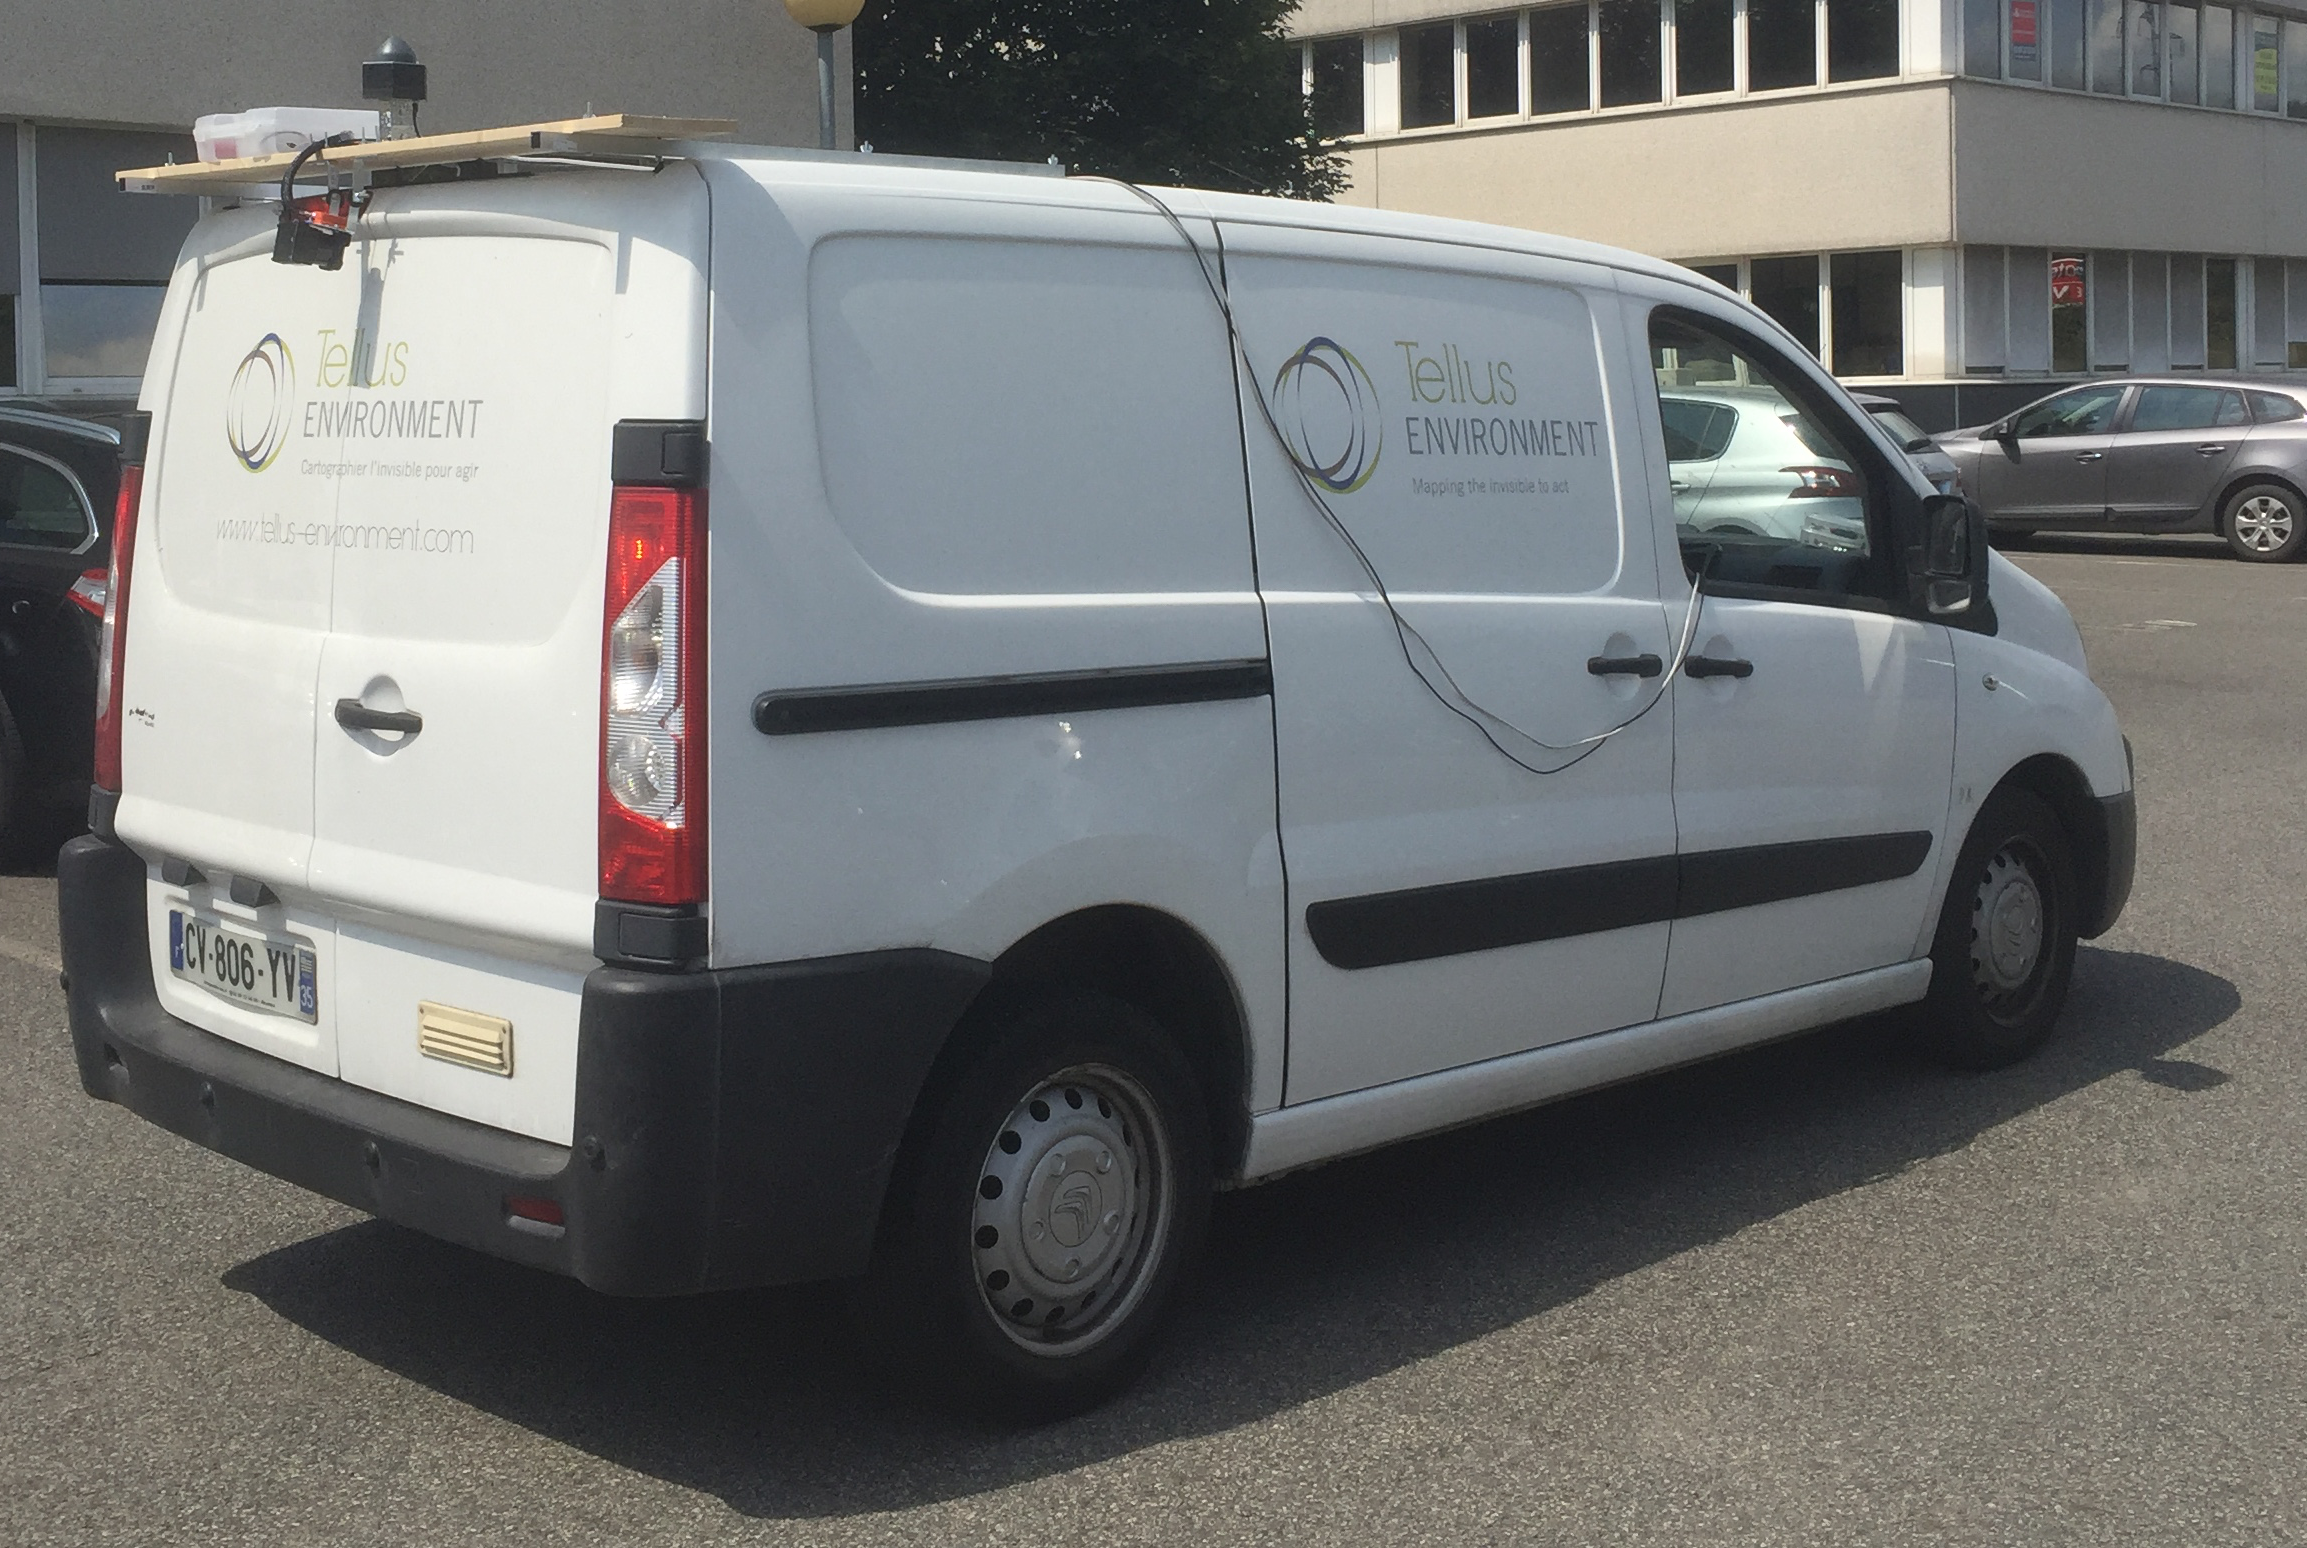
\includegraphics[width=0.7\linewidth]{img/telluscar}
		\caption[telluscar]{Telluscar avec capteurs montés à l'arrière}
		\label{fig:telluscar}
	\end{figure}

	\begin{figure}[h!]
		\centering
		\includegraphics[width=0.7\linewidth]{img/telluscardetail}
		\caption[telluscardetail]{Détail des capteurs monté l'arrière de la Telluscar.}
		\label{fig:telluscardetail}
	\end{figure}

	\para Le but des tests était de faire évoluer la Telluscar ainsi équipée en vue d'enregistrer simultanéement les données générées par l'IMU, le GPS et le LIDAR, pour ensuite les rejouer à posteriori et les soumettre à l'implémentation de Symeter V2.
	
	\subsection{Exploitation}
	\para Les données sont enregistrée en utilisant l'outil \verb|rosbag| de ROS qui permet d'enregistrer tous les topics diffusés lors d'une session de fonctionnement. L'outil \verb|rosbag| permet ensuite de rejouer ces captures et d'alimenter des nodes déployés indépendamment et ainsi les tester.
	
	\para C'est ainsi que l'on peut retrouver la trace des données GPS brutes extraites des captures (figure \ref{fig:trajectoire}), les données générées par l'IMU (figure \ref{fig:imelinacctine}), entre autre.
\begin{figure}[h!]
	\centering
	\includegraphics[width=1\linewidth]{img/trajectoire}
	\caption[trajectoire]{Exemple de trajectoire capturée par le GPS lors d'une capture de données}
	\label{fig:trajectoire}
\end{figure}


\begin{figure}[h!]
	\centering
	\includegraphics[width=0.7\linewidth]{img/imeLinAccTine}
	\caption[acclin]{Captures des accélérations linéaires issues de l'IMU XSens.}
	\label{fig:imelinacctine}
\end{figure}

	
	\section{Exploitation des données}
	\label{expdonnees}
	L'exploitation des données en vue de faire fonctionner le logiciel Symeter V2 à partir de données GPS, IMU et LIDAR enregistrées est en cours et n'a pas encore donné de résultat concluant.
	
	\para Deux difficultés sont rencontrées qui devront être levées pour permettre de reconstituer le trajet et l'évolution de la pose du véhicule dans le temps. Tout d'abord la pose de l'IMU par rapport au véhicule à l'air d'avoir une influence très importante sur le comportement du \verb|ekf_localization_node|. Si cette pose n'est pas exactement connue par le système Symeter V2, il est difficile de conserver une estimation fiable de la localisation. Ce problème n'était pas apparu dans la simulation car dans ce cas la pose du l'IMU simulé est implicitement connue avec précision.
	
	\para Le deuxième problème est que les données d'accélérations générées par l'IMU le sont selon un référentiel qui n'a pas l'air d'être celui attendu par \verb|ekf_localization_node|. Il faut donc rechercher quel référentiel est effectivement utilisé par l'IMU, corriger les données enregistrées de manière à compenser les incohérences d'orientation.
	
	\para Ce travail d'exploitation est donc encore en cours, mais une fois que ces problèmes auront été contournés, nous avons bon espoir de pouvoir générer un modèle 3D du parking à partir des captures LIDAR.
	 
\chapter{Perspectives}

Ce chapitre présente les perspectives d'évolution qui pourront être appliquées au projet Symeter V2. 

\section{Amélioration de l'utilisation de l'IMU}
Comme indiqué dans les chapitres précédents, le processus de localisation n'exploite pas encore pleinement les données d'accélération de l'IMU. L'intégration de ces données dans le \verb|ekf_localization_node| s'avère complexe et requiert une procédure d'exploitation particulière. 

\para L'une des pistes à explorer sera d'intégrer un module INS ("Inertial Navigation System", système de navigation inertiel) qui prendra en compte uniquement les données IMU pour générer son estimation propre de la pose. Cette pose serait ensuite soumise au \verb|ekf_localization_node| pour être fusionnée avec les informations GPS. Cela permettrait de séparer complètement la gestion de l'IMU de la fusion de données, et donc d'y voir plus clair quand à l'état de la localisation.

\section{Developpement d'un module d'accumulation propre à Symeter V2} 
Si le module \verb|octomap| a permis de monter le prototype initial de Symeter V2 pour la simulation sous Gazebo, et de démontrer la possibilité de faire l'acquisition d'un modèle numérique 3D d'un silo à partir d'un LIDAR mobile, ce module comporte quelques caractéristiques qui font qu'il n'est pas complètement adapté aux besoins de Symeter V2.

\para Notamment, le nuage de point généré par \verb|octomap| représente un information de présence de donnée dans un Voxel de 10x10cm, et le point généré est le barycentre du cube du voxel. Nous perdons donc de la précision dans la mesure d'altitude du tas d'ensilage.

\para Ceci nous forcera a développer un module d'accumulation et de stockage du modèle numérique 3D qui soit complètement adapté aux besoins de Symeter V2. 


\section{Simulation de l'action de tassage}
La simulation peut permettre la mise au point de la localisation, de l'acquisition initiale du chantier d'ensilage. Mais elle n'est pas directement utilisable pour simuler l'opération du tracteur dans le chantier d'ensilage. En effet il n'est pas possible de simuler physiquement le tassage à l'aide de Gazebo.

\para Il est cependant possible de mettre en oeuvre nos outils de manière à simuler logiquement l'évolution du chantier en implémentant un mécanisme de sauvegarde / restauration de l'état du chantier d'une session de fonctionnement à l'autre. En faisant varier la forme du tas d'ensilage simulé entre deux sessions, il sera possible d'émuler une action de tassage.

\section{Développement des outils de détection de monitoring de tassage}
Une fois les procédés d'acquisition d'un modèle numérique 3D à partir d'un LIDAR mobile finalisés, nous pourrons commencer à mettre en place le monitoring du tassage lui-même.

\para Ce monitoring devra comparer les modifications du modèle numérique au fur-et-à-mesure de la progression du chantier, enregistrer l'évolution au cours du temps du silo, générer les données d'aide à la décision.

\para Une interface homme/machine permettant de piloter l'intervention du système Symeter V2 sur le chantier devra aussi être développée. 


\chapter{Conclusion}

Au cours de ce stage, nous avons pu confirmer que les outils de simulation proposés par les environnements  ROS et Gazebo pouvait permettre le développement du produit Symeter V2, qualitativement et quantitativement.

\para Nous avons pu implémenter une plateforme de test simulée sous Gazebo et l'environnement physique virtuel associé, permettant ainsi d'émuler le chantier d'ensilage, le tracteur et le système Symeter V2 monté sur celui-ci.

\para Nous avons mis en place le système de localisation en mettant en oeuvre un composant pré-éxistant de fusion de capteurs, \verb|ekf_robot_localization|, et ainsi exploiter des signaux de l'IMU et du GPS. Ceci nous permet d'obtenir la pose du véhicule avec une précision compatible avec un reconstitution qualitative du chantier simulé. Nous avons aussi développé les scripts permettant de vérifier le bon fonctionnement de ce procédé.

\para Nous avons mis en place la chaine d'acquisition des données Lidar en utilisant principalement les composants disponibles dans Point Cloud Library. Nous avons prétraité ces données en convertissant le format angles/distance en un nuage de points préliminaire, et nous avons filtré ce nuage de points de manière à répartir régulièrement les points de mesure et réduire le flot de données à traiter.

\para Nous avons enfin mis en oeuvre le composant \verb|OctoMap| pour effectuer l'accumulation des données LIDAR acquises. Nous générons ainsi un nuage de points 3D représentant notre chantier d'ensilage simulé. Nous validons ainsi la faisabilité de Symeter V2.

\para Nous avons aussi tenté d'utiliser le prototype de Symeter V2 pour exploiter des captures réelles. Ce travail est encore en cours.

\para Nous avons pu dégager des axes d'amélioration pour augmenter la précision de la localisation, obtenir un nuage de points représentant plus fidèlement le chantier. L'objectif de ces améliorations est d'accéder à un niveau de qualité du procédé qui permette des mesures précises du tassage et du volume.

\para Nous avons donc à l'issue de ce stage une plateforme fondamentale de simulation qui va permettre à Tellus Environment de développer les fonctionnalités de mesures du tassage de silo et de mesure de volume du système Symeter V2. 

\para Cette plateforme simulée va aussi permettre à Tellus Environment de tester virtuellement diverses configurations de capteurs et ainsi permettre de mieux définir le contour du produit. Cela permet à Tellus Environment d'envisager que les premiers tests en grandeur du système Symeter V2, au cours de vrais chantiers d'ensilage, se dérouleront de manière productive.

\para L'avenir du projet Symeter V2 est en cours de détermination par ses commenditaires, avec une forte probabilité de continuer pour au moins un an supplémentaire. Cette année sera consacrée au montage d'un prototype fonctionnel et de la conduite des tests en grandeur. Tellus Environment m'a proposé de continuer l'aventure, et nous sommes tombés d'accord pour mener à bien ensemble ce projet dans le cadre d'un CDD d'un an.



\begin{appendix}
	\chapter{Représentation de l'Attitude et des Rotations}
	\label{app:a}
	Selon \cite{gustavsson_uav_2015}, si nous considérons un véhicule mesurant des mouvements par rapport à son propre repère et un autre système mesurant les positions et vitesses etc du même véhicule par rapport à un repère $\{e\}$, et si la navigation est effectuée par rapport à un repère local de navigation ${n}$, il devient très vite apparent qu'un outil pour décrire l'orientation du véhicule par rapport à ces différents repères est nécessaire.
	
	\para Deux des manières les plus communes de représenter les attitudes et les rotations dans $\mathbb{R}^3$ sont les \textit{Angles d'Euler} et les \textit{quaternions}.
		\section{Angles d'Euler}
		Selon \cite{nuchter_3d_2009}, alors que les trois coordonnées Cartesiennes $x,y$ et $z$ représentent la position, les trois angles $\theta_x$, $\theta_y$ et $\theta_z$ décrivent l'orientation dans $\mathbb{R}^3$. L'union de la position et de l'orientation est appelée la \textit{pose}. L'orientation $\theta_x$, $\theta_y$ et $\theta_z$ est la rotation autour des axes principaux du repère orthonormé, c'est à dire $(1,0,0)$, $(0,1,0)$ et $(0,0,1)$. Les matrices de rotation sont les suivantes:
		
		\begin{equation*}
		\bs{R}_x =	\begin{pmatrix}
		1 & 0 & 0 \\
		0 & \cos{\theta_x} & -\sin{\theta_x}\\
		0 & \sin{\theta_x} & \cos{\theta_x}
		
		\end{pmatrix}
		\end{equation*}
		
		\begin{equation*}
		\bs{R}_y = \begin{pmatrix}
		\cos{\theta_y} & 0 & \sin{\theta_y}\\
		0 & 1 & 0 \\
		-\sin{\theta_y} &  0 & \cos{\theta_y}
		\end{pmatrix}
		\end{equation*}
		
		\begin{equation*}
		\bs{R}_z = \begin{pmatrix}
		\cos{\theta_z} & -\sin{\theta_z}& 0 \\
		\sin{\theta_z} & \cos{\theta_z} & 0 \\
		0 & 0 & 1
		\end{pmatrix}
 		\end{equation*}
 		
 		\para La matrice de rotation globale est calculée comme $\bs{R} = \bs{R}_{\theta_x, \theta_y, \theta_z} = \bs{R}_x \bs{R}_y \bs{R}_z$.
 		
 		\para Note: La matrice ci-dessus dépend de l'ordre de la multiplication. Des matrices de rotation différentes sont obtenues par $\bs{R} = \bs{R}_{\theta_z, \theta_y, \theta_x} = \bs{R}_z \bs{R}_y \bs{R}_x$ ou $\bs{R} = \bs{R}_{\theta_y, \theta_x, \theta_z} = \bs{R}_y \bs{R}_x \bs{R}_z$. De plus un blocage de cardan peut intervenir si les axes 
		
		\section{Quaternions Unitaires}
		Toujours selon \cite{nuchter_3d_2009}, les quaternions sont un nombre complexe à 4 dimensions qui peuvent être utilisés pour représenter des rotations en 3D. Ils sont générés en postulant une racine additionnelle à -1 nommée $j$ qui ne soit pas $i$ ou $-i$. Il existe alors nécessairement un élément $k$ tel que $ij = k$ qui aussi une racine de -1. Les relations suivantes sont aussi vraies:
		

		\begin{equation*}
		\begin{aligned}
			i^2&= j^2 & = k^2 = i&jk &=& -1 \\
			ij &= k, &           &ji &=& -k \\
			jk &= i,&            &kj &=& -i \\
			ki &=j, &            &ik &=& -j
		\end{aligned}
		\end{equation*}
		
		\para $i,j,k$ et -1 forment la base du quaternion $\mathbb{H}$. Tout quaternion $\bs{\dot{q}}$ peut être représenté sous la forme $\bs{\dot{q}} = q_0 + q_xi + q_yj+q_zk$. Ainsi tout quaternion définit un unique 4-vecteur $(q_0, q_x, q_y, q_z)^T \in \mathbb{R}^4$. 
		
		\para Comme pour les nombres complexes, les quaternions possèdent un unique quaternion conjugué. Le quaternion conjugué de $\bs{\dot{q}} = q_0 + q_xi + q_yj+q_zk$ est $\bs{\dot{q}}^\ast = q_0 - q_xi - q_yj-q_zk$.
		
		\para En utilisant le quaternion conjugué et le produit scalaire, nous pouvons calculer la norme du quaternion $\bs{\dot{q}}$:
		
		\begin{equation*}
		\|\bs{\dot{q}}\| = \sqrt{\langle \bs{\dot{q}}, \bs{\dot{q}}^{\ast} \rangle} = \sqrt{q_0^2 + q_x^2 + q_y^2 + q_z^2}
		\end{equation*} 
		
		\para Le sous-ensemble des quaternions unité est important car ses éléments peuvent représenter les rotations dans $\mathbb{R}^3$. Un quaternion unité $\bs{\dot{q}}$	vérifie la relation $\|\bs{\dot{q}}\| = 1$. Un quaternion unité a pour propriété que sont inverse $\bs{\dot{q}}^{-1}$ est égal à son conjugué $\bs{\dot{q}}^\ast$.
		
		\begin{equation*}
		\langle \bs{\dot{q}}, \bs{\dot{q}}^{\ast} \rangle = \|\bs{\dot{q}}\|^2 = 1
		\end{equation*}
		
		\para Les rotations utilisant les quaternions sont formalisées comme suit: soit $\bs{\dot{q}}$ tel que $\bs{\dot{q}} = (q_0,q_x,q_y,q_z) = (q_0,\bs{q})$. Pour effectuer la rotation du point 3D $\bs{p}=(p_x,p_y,p_z)^T \in \mathbb{R}^3$, nous écrivons ce point sous la forme d'un quaternion aussi: $\bs{\dot{p}} = (0, p_x,p_y,p_z)^T = (0,\bs{p})$. Alors nous pouvons démontrer que le point $p_{\mathrm{rot}}$ est le résultat d'une rotation du point $\bs{p}$ par la formule
		
		\begin{equation*}
		\bs{p}_{\mathrm{rot}} = \bs{\dot{q}\dot{p}\dot{q}}^{\ast}
		\end{equation*}
		
		\para \cite{nuchter_3d_2009} montre qu'une rotation d'un angle $\theta$ autour d'un vecteur $\bs{n}$ sera représenté par le quaternion 
		
		\begin{equation*}
			\bs{\dot{q}} = \left( \cos{\frac{\theta}{2}}, \sin{\frac{\theta}{2}}\bs{n} \right)
		\end{equation*}
		
		\para Pour passer d'une représentation en quaternion en une représentation de rotation autour d'un axe, il suffit de calculer les composantes suivantes:
		
		\begin{equation*}
		\begin{aligned}
			\theta 	&= 2 \arccos{q_0} \\
			n_x 	&= \frac{q_x}{\sin{\theta}} \\
			n_y		&= \frac{q_y}{\sin{\theta}} \\
			n_z		&= \frac{q_z}{\sin{\theta}} 
		\end{aligned}
		\end{equation*}

\end{appendix}

\nocite{*}
\bibliographystyle{alpha}
\bibliography{biblio}

\end{document}